\chapter{Data Management}
\label{cha:dms}
\Authors{Carolin Helbig, Uwe-Jens G\"orke, Mathias Nest, Daniel P\"otschke, Amir S. Sattari, Patrick Schmidt, Bernhard Vowinckel, Keita Yoshioka, Olaf Kolditz}

Data management includes the development and use of architectures, guidelines, practices and procedures for accurate managing of data during the entire data lifecycle of an institutional unit or a research project. Data are defined as different information units such as numbers, alphabetic characters, and symbols that are particularly formatted and can be processed by computer. The data in the project is provided by various actors which can be GeomInt partners, their legal representatives, employees, and external partners. GeomInt Data is provided at GeomInt data management portal (DMP).

In GeomInt project the partners work is very close cooperation. Project-owned and connected infrastructures are synergetic used (as illustrated in Fig. \ref{fig:geomint-dms}). In addition to the rock mechanics laboratories of the partners CAU, IfG and TUBAF with partly unique equipment data from ongoing experiments in the underground laboratories are accessed. An essential element of the GeomInt project is the simulation and software development structures illustrated in Fig. \ref{fig:geomint-dms}. With regard to the use of the simulation platform OpenGeoSys, the development of which is coordinated by the UFZ and in whose further development the GeomInt partners BGR, CAU, IfG and TUBAF are involved, the simulation and development infrastructures located at the UFZ, including version management, is available to these partners. 

%\begin{figure}{l}{\textwidth}
\begin{figure}
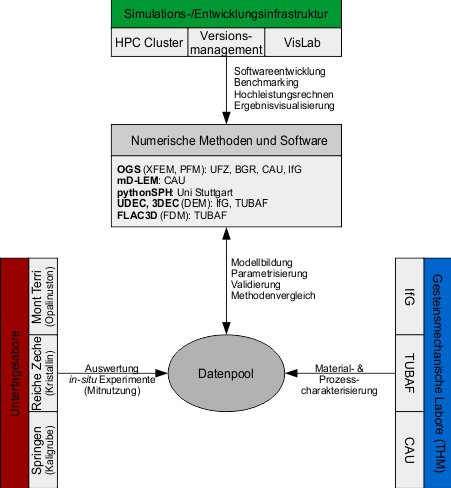
\includegraphics[width=\textwidth]{figures/geomint-dms.png}
\caption{Network diagram to illustrate synergies and dependencies in the GeomInt network in connection with the infrastructure elements and numerical methods in the project}
\label{fig:geomint-dms}
\end{figure}

The collaborative work requires data management structures and guidelines. Therefore, the first step was to set up a document that includes a user agreement and a data management plan which is the basis for data management in the project.

% The synergetic use of project-owned and connected infrastructures is illustrated in Fig. \ref{fig:geomint-dms}. In addition to the rock mechanics laboratories of the partners CAU, IfG and TUBAF with partly unique equipment (e.g. large shear apparatus of TUBAF, crack detection by means of sound waves by CAU and TUBAF, especially triax cells for percolation experiments at high temperatures at IfG), data from ongoing experiments in the above-mentioned underground laboratories are accessed. An essential element of the GeomInt project is the simulation and software development structures illustrated in Fig. \ref{fig:geomint-dms}. With regard to the use of the simulation platform OpenGeoSys, the development of which is coordinated by the UFZ and in whose further development the GeomInt partners BGR, CAU, IfG and TUBAF are involved, the simulation and development infrastructures located at the UFZ, including version management, is available to these partners.

% The immediate project results include specific data from laboratory and in-situ experiments, software components and data sets from numerical simulations (i.e. model and result files). An estimation of the extent of the data generated in GeomInt is variable; therefore, the data management concept must be flexible. This uncertainty is mainly due to the fact that the evaluation of test and calculation results may lead to a change in test and calculation planning and may even lead to additional experiments or simulation calculations. As a measure for the expected orders of magnitude, however, it is possible, for example, to estimate the size of the data set (input and output data) for the three-dimensional simulation of a transient coupled process in relation to an in-situ experiment (small field scale) with a gigabyte amount in the low two-digit range. A total data volume in the terrabyte range therefore must be manageable.

% The availability of experimental and numerical data generated in the project, including existing metadata, is realised for the project partners in an internal area of the Geomint homepage. The Helmholtz Centre for Environmental Research - UFZ is responsible for the project data. The UFZ has many years of experience in data management regarding the cooperative development of open source software (OpenGeoSys) as well as the acquisition, storage and processing of data from experiments on different scales, exploration and monitoring campaigns, numerical simulations and scientific 3D visualisations. The UFZ has sufficient capacities and modern data management systems for data storage, which are available as a central data infrastructure for the planned research network. Specifically, data sets are managed by means of an ORACLE database. Access is via a web portal, where each data record must be provided with metadata before uploading. The metadata standard used is compatible with the INSPIRE Directive 2007/2/EC and also regulates the rights for access, use and transfer of the data. A tape system is also available for the long-term storage of very large amounts of data. For the provision of exploration and monitoring data, geo-services mentioned in the GDI-DE are used as far as possible (e.g. Sensor Observation Service or Web Map Service). Since such services for complex modelling and simulation data do not exist so far, the provision is done via a data research portal, where data can be found by means of stored metadata. 

% As software components are part of non-commercial, scientific program platforms and are open source products (e.g. OpenGeoSys), they are hosted by the responsible partner via established source code hosting services (e.g. GitHub) is made publicly available. A possible public access to project data, which goes beyond the status quo as described in technical publications, as well as the handling of the data after the end of the project is regulated in the cooperation agreement or in the cooperation contract between the project partners. The handling of data obtained from the in-situ experiments in the underground laboratories through synergies with other projects is also regulated separately (access authorisation for these data, storage location, publication, handling of the data after the end of the project). Such an approach is necessary because specific parts of these data can be used for the scientific purposes of GeomInt, but they are generated in other projects with partly other partners.

\section{User agreement and data management plan}

The GeomInt project partners agreed to set up a user agreement which includes specifications for data structures including metadata, data formats, access authorization for data, the possible publication of data, as well as the handling of the data after the end of the project and outside the project. A first version of this user agreement was created six months after the start of the project. 

The user agreement includes guidelines and definitions for the following aspects 

\begin{list}{-}{\leftmargin=1em \itemindent=0em \itemsep=0.2em}
\item Which data will be generated in the project and has to be managed?
\item How will data be provided and exchanged?
\item What are the rights of use for the partners and for third parties?
\item How to cite data?
\item How to supervise the compliance of the user agreement?
\end{list}

As part of the user agreement, a data management plan, which is a formal document that describes how project data is managed during the research period and after completion of the project, was developed. The goal of a DMP plan is to consider the aspects of data management (metadata creation, data preservation and analysis) before the start of the project. Following points are discussed in the GeomInt DMP:

\begin{enumerate}{\leftmargin=1em \itemindent=0em \itemsep=0.2em}
\item Generation and management methods (data infrastructure, external data, data integration, data formats, quality control, user groups, data processing stages, versioning, documentation and meta data, geocoding)
\item Data Legal Management
\item Data exchange and provision, citation rules
\item Short-term storage and data management (storages, data transfer, backup, security)
\item Long-term storage (characteristics, metadata and documentation, responsibility)
\item Resources (organizational roles and responsibilities for data management)
\end{enumerate}

\section{GeomInt data}

The project results include specific data from laboratory and in-situ experiments, software components and data sets from numerical simulations (i.e. model and result files). An estimation of the extent of the data generated in GeomInt could not be made before the project. Therefore, the data management concept had to be flexible. This uncertainty was mainly due to the fact that the evaluation of test and calculation results may lead to a change in test and calculation planning and may even lead to additional experiments or simulation calculations. 

The availability of experimental and numerical data generated in the project, including existing metadata, is realized on an internal area of the Geomint homepage. The Helmholtz Centre for Environmental Research - UFZ is responsible for the project data. The UFZ has many years of experience in data management regarding the cooperative development of open source software (OpenGeoSys) as well as the acquisition, storage and processing of data from experiments on different scales, exploration and monitoring campaigns, numerical simulations and scientific 3D visualizations. 

The UFZ has sufficient capacities and modern data management systems for data storage, which are available as a central data infrastructure for the planned research network. Specifically, data sets are managed by means of an ORACLE database. Access is via a web portal, where each data record must be provided with metadata before uploading. The metadata standard used is compatible with the INSPIRE Directive 2007/2/EC and also regulates the rights for access, use and transfer of the data. A tape system is also available for the long-term storage of very large amounts of data. For the provision of exploration and monitoring data, geo-services mentioned in the GDI-DE are used as far as possible. Since such services for complex modelling and simulation data do not exist so far, the provision is done via a data research portal, where data can be found by means of stored metadata.

As software components are part of non-commercial, scientific program platforms and are open source products (e.g. OpenGeoSys), they are hosted by the responsible partner via established source code hosting services (e.g. GitHub) is made publicly available. A possible public access to project data, which goes beyond the status quo as described in technical publications, as well as the handling of the data after the end of the project is regulated in the cooperation agreement or in the cooperation contract between the project partners. 

The handling of data obtained from the in-situ experiments in the underground laboratories through synergies with other projects is also regulated separately (access authorisation for these data, storage location, publication, handling of the data after the end of the project). Such an approach is necessary because specific parts of these data can be used for the scientific purposes of GeomInt, but they are generated in other projects with partly other partners.

\begin{figure}[!ht]

\includegraphics[width=\textwidth]{figures/geomint-web-01.png}
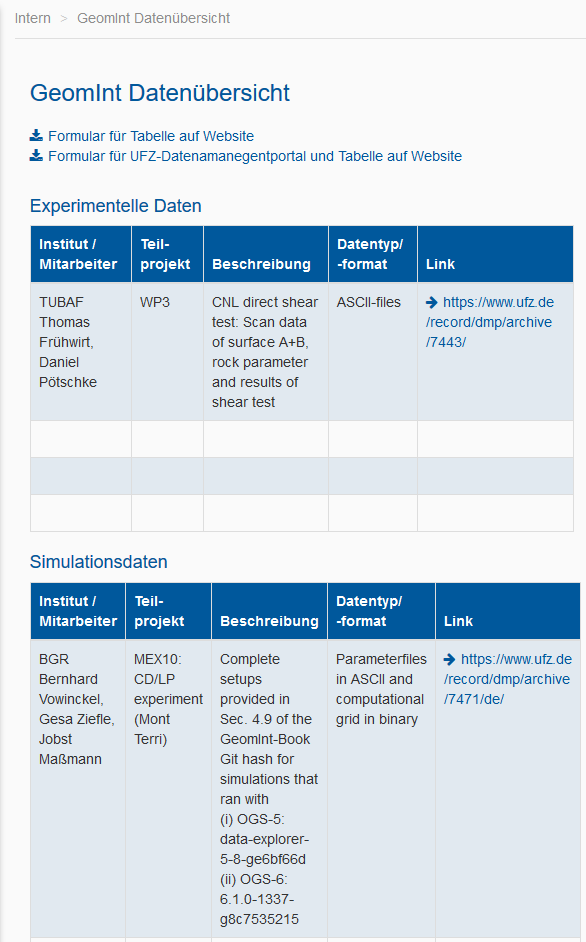
\includegraphics[width=\textwidth]{figures/geomint-web-02.png}
\caption{GeomInt DMS Portal}
\label{fig:geomint-web}
\end{figure}

\section{GeomInt DMP}

In this section, exemplary data sets of every project partner are described. A table of these data sets including description and link are available only for project partners at the website (Fig. \ref{fig:geomint-web}). Some data sets can be found on the UFZ data investigation portal \hyperlink{https://www.ufz.de/drp/}{https://www.ufz.de/drp/}. These data sets are uploaded to the data management portal at UFZ (DMP@UFZ).

\begin{table}[!ht]
\footnotesize
\centering
\caption{MEX Data Management}
\label{tab:dms-mex}
\begin{tabular}{|C{0.6cm}|L{3.7cm}|C{0.7cm}|C{0.7cm}|C{0.7cm}|C{0.7cm}|C{0.7cm}|C{0.7cm}|} 
\hline 
\rowcolor{cyan!50}
MEX & TOP & EXP & \multicolumn{5}{c|}{MOD} \\ 
\hline
\rowcolor{cyan!50}
WP &  &  & LEM & DEM & FEM1 & FEM2 & FFS \\ 
\hline \hline
%-------------------
0-1a & Bending fracture test & REF & \cellcolor{yellow} \checkmark & \cellcolor{yellow} \checkmark & \cellcolor{yellow} \checkmark &  &  \\ 
\hline 
0-1b & Bending fracture test (aniso) & \cellcolor{yellow} & \cellcolor{yellow} & \cellcolor{yellow} & \cellcolor{yellow} &  &  \\ 
\hline 
0-2 & Humidity controlled bending & \multicolumn{6}{c|}{Concept} \\ 
\hline \hline
%-------------------
1-1a & Swelling of clay & \cellcolor{yellow} & \cellcolor{yellow} & \cellcolor{yellow} & \cellcolor{yellow} &  &  \\ 
\hline
1-1b & Swelling of clay & \cellcolor{yellow} &  & \cellcolor{yellow} &  &  &  \\ 
\hline
1-2 & Shrinkage of clay & \cellcolor{yellow} & \cellcolor{yellow} & \cellcolor{yellow} & \cellcolor{yellow} &  &  \\ 
\hline
1-3 & Desiccation of clay & \cellcolor{yellow} &  &  &  &  &  \\ 
\hline
1-4 & CD/LP experiment &  &  &  & \cellcolor{green} &  &  \\ 
\hline \hline
%-------------------
2-1a & Pressure driven percolation &  & \cellcolor{yellow} & \cellcolor{yellow} & \cellcolor{green} &  &  \\ 
\hline
2-1b & Pressure driven percolation & \cellcolor{yellow} & \cellcolor{yellow} & \cellcolor{yellow} & \cellcolor{yellow} &  &  \\ 
\hline
2-2 & Healing / closure & \cellcolor{yellow} & \cellcolor{yellow} & \cellcolor{yellow} & \cellcolor{yellow} &  &  \\ 
\hline
2-3 & Compressible fluids & \cellcolor{yellow} & \cellcolor{yellow} & \cellcolor{yellow} &  &  &  \\ 
\hline
2-4 & URL Springen & \cellcolor{yellow} &  & \cellcolor{yellow} &  &  &  \\ 
\hline \hline
%-------------------
3-1 & CNL test & \cellcolor{green} &  &  &  &  & \cellcolor{green} \\ 
\hline
3-2 & CNS test & \cellcolor{green} &  &  &  &  & \cellcolor{green} \\ 
\hline
3-3 & Cyclic loading &  &  &  &  & \cellcolor{yellow} &  \\ 
\hline \hline
%-------------------
\end{tabular}
\end{table}
\normalsize

\subsection{Software Codes}
\begin{list}{-}{\leftmargin=1em \itemindent=0em \itemsep=0em}
\item LEM: in-house code
\item DEM: commercial code by Itasca Ltd.
\item SPH: in-house code
\item OGS (OpenGeoSys): \url{https://www.opengeosys.org/releases/}
\item FEM@UoS: 
\end{list}
\subsection{Input files}
\begin{list}{-}{\leftmargin=1em \itemindent=0em \itemsep=0em}
\item LEM: in-house code
\item DEM: Itasca Ltd. (user's manuals)
\item SPH: in-house code
\item OGS (Benchmarks): \url{https://www.opengeosys.org/docs/benchmarks/}
\item FEM@UoS: in-house code
\end{list}

\clearpage
%------------------------------------------------------------------------
\subsection{MEX 0-1a: Bending fracture test}

\subsubsection*{CAU Kiel}

The required LEM code and the input variables of the three-Point fracture toughness test on the Rockville Granite samples are uploaded to the IfG (Kiel) NextCloud server. The data is accessible through the following link:\\
\hyperlink{https://nextcloud.ifg.uni-kiel.de/index.php/s/pRmBPJ9gK5Se6ci}{https://nextcloud.ifg.uni-kiel.de/index.php/s/pRmBPJ9gK5Se6ci}\\

The uploaded protected MATLAB file in a *.p format requires a MATLAB version with a built-in Voronoi Tessellation and Delaunay Triangulation functions. The input variables are prepared in a single file for the simulation of the fracture toughness in Rockville Granite. Figure \ref{fig:Amir_ME1_LEM_Displacement_Crystalline_Data} shows the relation between the load vs. CMOD as described in section \ref {sec:mex01}.

\begin{figure}[!ht]
\centering
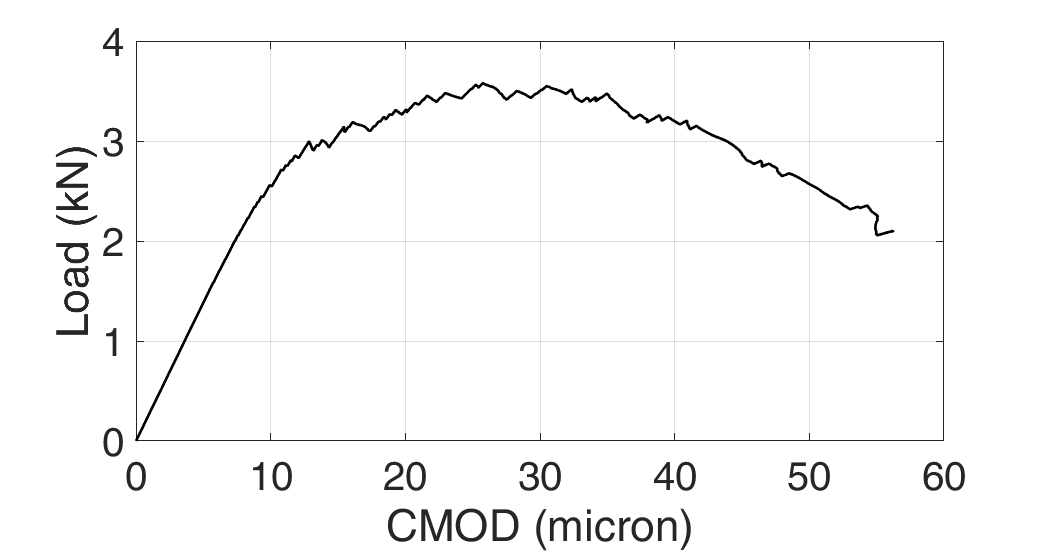
\includegraphics[width=0.75\textwidth]{figures/Amir_ME1_LEM_Displacement_Crystalline_Data.png}
\caption{The load vs. CMOD from the lattice simulation}
\label{fig:Amir_ME1_LEM_Displacement_Crystalline_Data}
\end{figure}

\begin{table}[!ht]
\caption{MEX 0-1a: Bending fracture test}
\label{tab:dms-mex0-1a}
\small
\begin{tabular}{R{3cm}|L{7cm}}
\hline
%
Data label & GeomInt | CAU | Bending fracture test, Granite \\
URI &  https://nextcloud.ifg.uni-kiel.de/index.php/s/pRmBPJ9gK5Se6ci (Numerics)\\
Subject  &  Bending fracture test, Granite\\
Type of data  &  executable MATLAB P-file, input parameters\\
Dataquality  &  quality assured data \\
Status of data  &  unprocessed data\\
Dataformat  & txt, MATLAB executable P-file\\
Creators  &  Kiel University, Institute of Geomechanics and Geotechnics, Ludewig-Meyn-Stra\ss e 10, 24118, Kiel\\
Source/Origin & In-house code \\
Publisher  &  Kiel University, Institute of Geomechanics and Geotechnics, Ludewig-Meyn-Stra\ss e 10, 24118, Kiel \\
Rights holders &  Kiel University, Institute of Geomechanics and Geotechnics, Ludewig-Meyn-Stra\ss e 10, 24118, Kiel \\
Contributors &   Kiel University, Institute of Geomechanics and Geotechnics: Amir Shoarian Sattari, Frank Wuttke\\
Time or Period of creation &  2018-2019\\
Language of the content &  English\\
Update policy &  stored data is final\\
Access permissions & full access\\
%
\hline
\end{tabular}
\end{table}

\subsubsection*{UFZ}
The source code can be found in OpenGeoSys project on github and  the input files for the three point bending test performed on the Rockville Granite samples have been uploaded.
The files include the unstructured finite element mesh files in vtu format and an OGS input file in xml format.
As homogeneous properties such as Youngu's modulus are assigned int the computational domain, the spatially constant material properties are specified in the OGS input file rather than in the mesh file.
The load and crack mouth opening displacment computed from the simulations are shown in~\ref{fig:Keita_ME1_VPF_Rockville} as described in section \ref {sec:mex01}.

\begin{figure}[!ht]
\centering
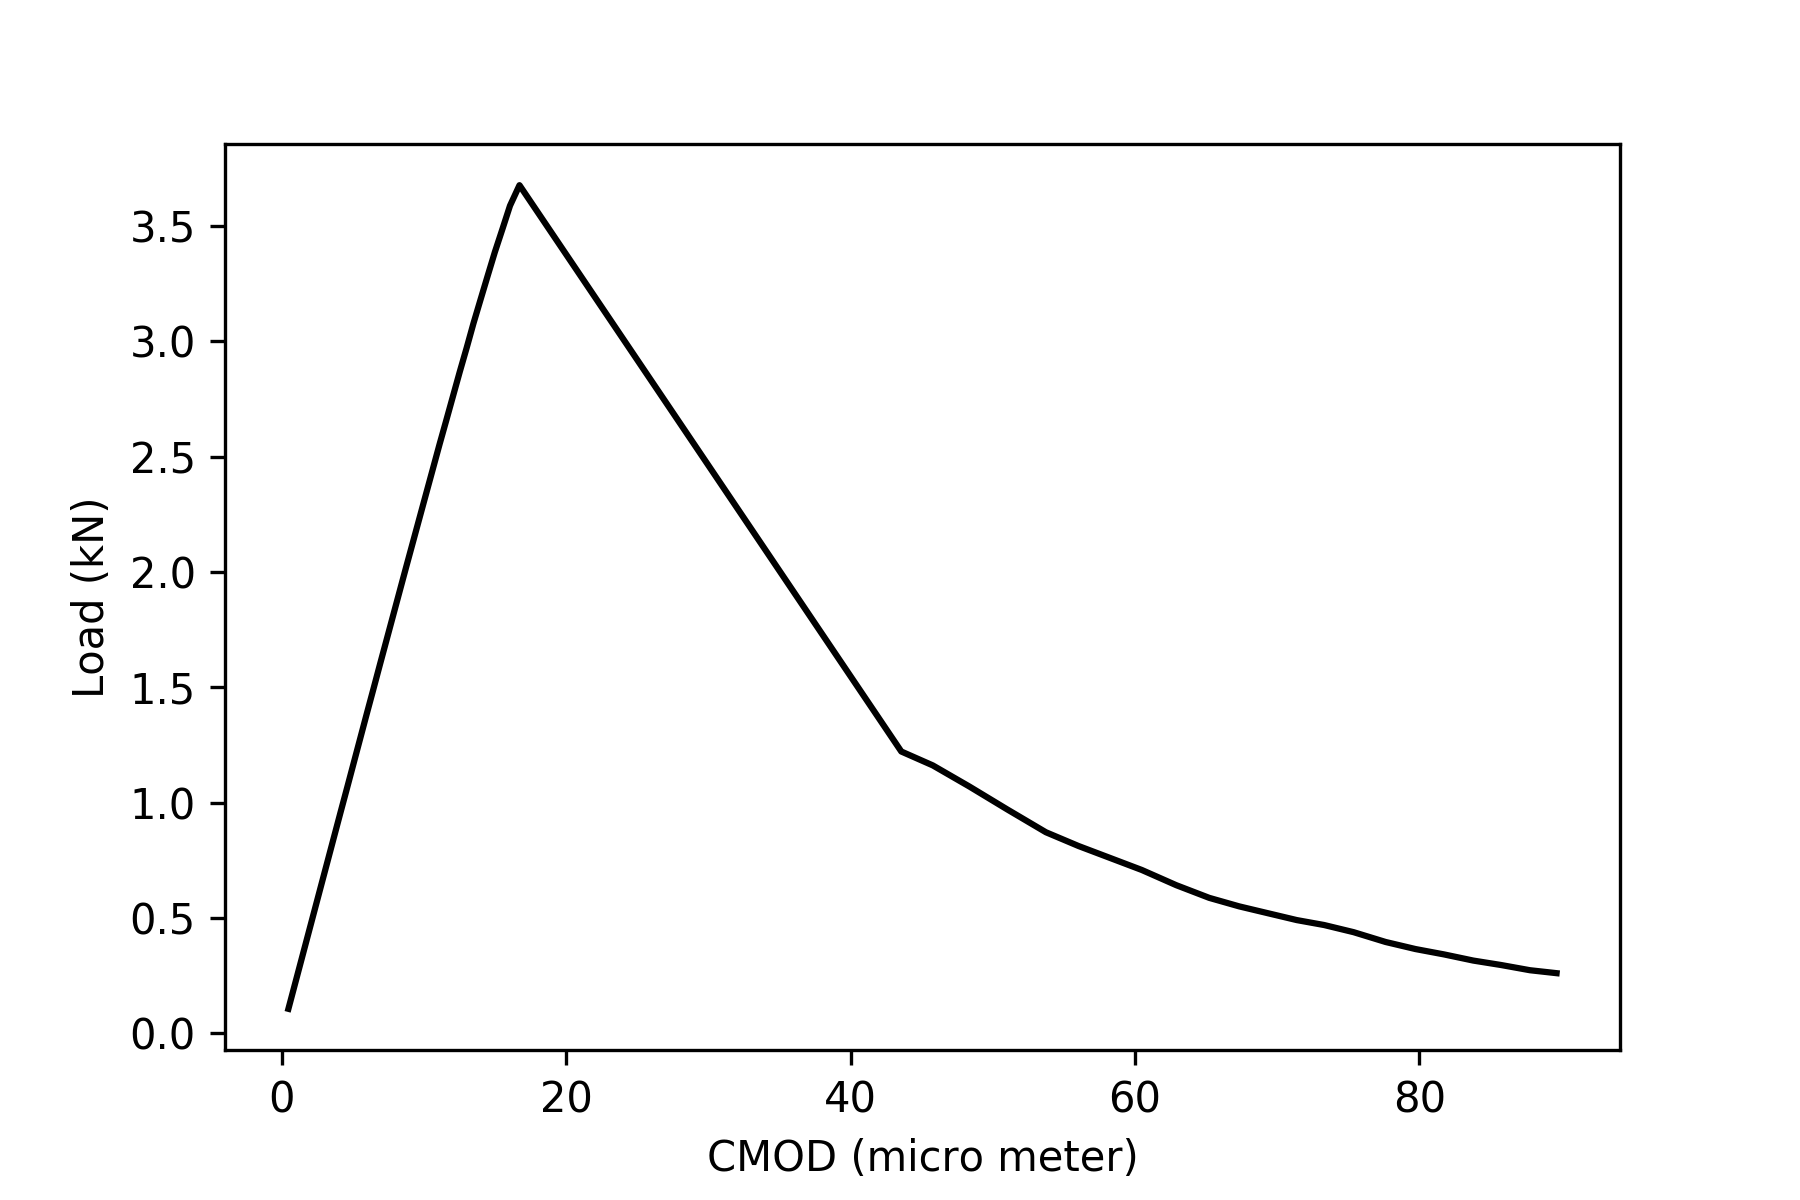
\includegraphics[width=0.75\textwidth]{figures/VPF_ME1_NF_CMOD.png}
\caption{The load vs. CMOD from the VPF simulation results}
\label{fig:Keita_ME1_VPF_Rockville}
\end{figure}

\subsubsection*{IfG}

Data management for MEX 0-1a (see section \ref{sec:mex01} for Model-Experiment description).

\todo[inline]{[UFZ](KY): Please add a template for OGS-6 (e.g. \url{https://www.opengeosys.org/docs/benchmarks/phase-field/phasefield/})}
\todo[inline]{The branch is not merged with the master yet. Files have been provided to datamanagement.}

\begin{table}[!ht]
\caption{MEX 0-1a: Meta Data according to Dublin Core}
\label{tab:dms-mex0-1a}
\small
\begin{tabular}{R{3cm}|L{7cm}}
\hline
%
Data label &  \\
URI &  \\
Subject  &  \\
Type of data  &  \\
Dataquality  &  \\
Status of data  &  \\
Dataformat  & \\
Creators  &  \\
Source/Origin &  \\
Publisher  &  \\
Rights holders &  \\
Contributors &  \\
Time or Period of creation &  \\
Language of the content &  \\
Update policy &  \\
Access permissions &  \\
%
\hline
\end{tabular}
\end{table}
\clearpage
%------------------------------------------------------------------------
\subsection{MEX 0-1b: Three-Point fracture toughness test, Opalinus Clay}

Participating institutions of MEX 0-1b (see section \ref{sec:mex01b}): CAU, UFZ

\begin{table}[ht!]
\caption{MEX 0-1b: Data overview}
\label{tab:dms-mex01b-overview}
\small
\begin{tabular}{l|l|l|l|L{4.7cm}}
\hline
\rowcolor{cyan}
Type & Spec. & Owner & Access     & Comment                       \\ 
\hline
EXP  &   Ben    & CAU   & Open    & Output files are uploaded     \\
\hline \hline
MOD  & LEM   & CAU   & Open       & Executable MATLAB P-file      \\
     &       &       & Open       & Input files will be uploaded  \\
\hline
MOD  & FEM   & UFZ   & Open       & Branch to be merged into OGS  \\
     &       &       & Open       & Input files available         \\
%
\hline
\end{tabular}
\end{table}
\normalsize

\subsubsection*{CAU Kiel}

The experimental results of the three-point fracture toughness test on the Opalinus Clay samples are uploaded to the IfG (Kiel) NextCloud server. The data is accessible through the following link:\\
\url{https://nextcloud.ifg.uni-kiel.de/index.php/s/pJxp2eNEJb6PfiS}

The data set, which includes the time, applied force ($N$) and the displacement of the sample at the loading point ($mm$), is provided in a *.txt file. The crack mouth opening displacement (CMOD), which is determined from the image processing technique (section \ref {sec:Fracture_Toughness_Exp}), is given in a *.xlsx file. The data includes the time and the calculated CMOD (mm). 

The required LEM code and the input variables of the three-Point fracture toughness test on the Opalinus Clay samples are uploaded to the IfG (Kiel) NextCloud server. The data is accessible through the following link:\\
\url{https://nextcloud.ifg.uni-kiel.de/index.php/s/ZBFN2rSZ99kPY9M}

The uploaded protected MATLAB file in a *.p format requires a MATLAB version with a built-in Voronoi Tessellation and Delaunay Triangulation functions. The input variables are prepared in two different files for a parallel and perpendicular embedded layer orientations. Figure \ref{fig:Amir_ME1_LEM_Claystone_Data} shows the comparison between the experimental and numerical data as described in section \ref {sec:mex01b}.

\begin{figure}[!ht]
\centering
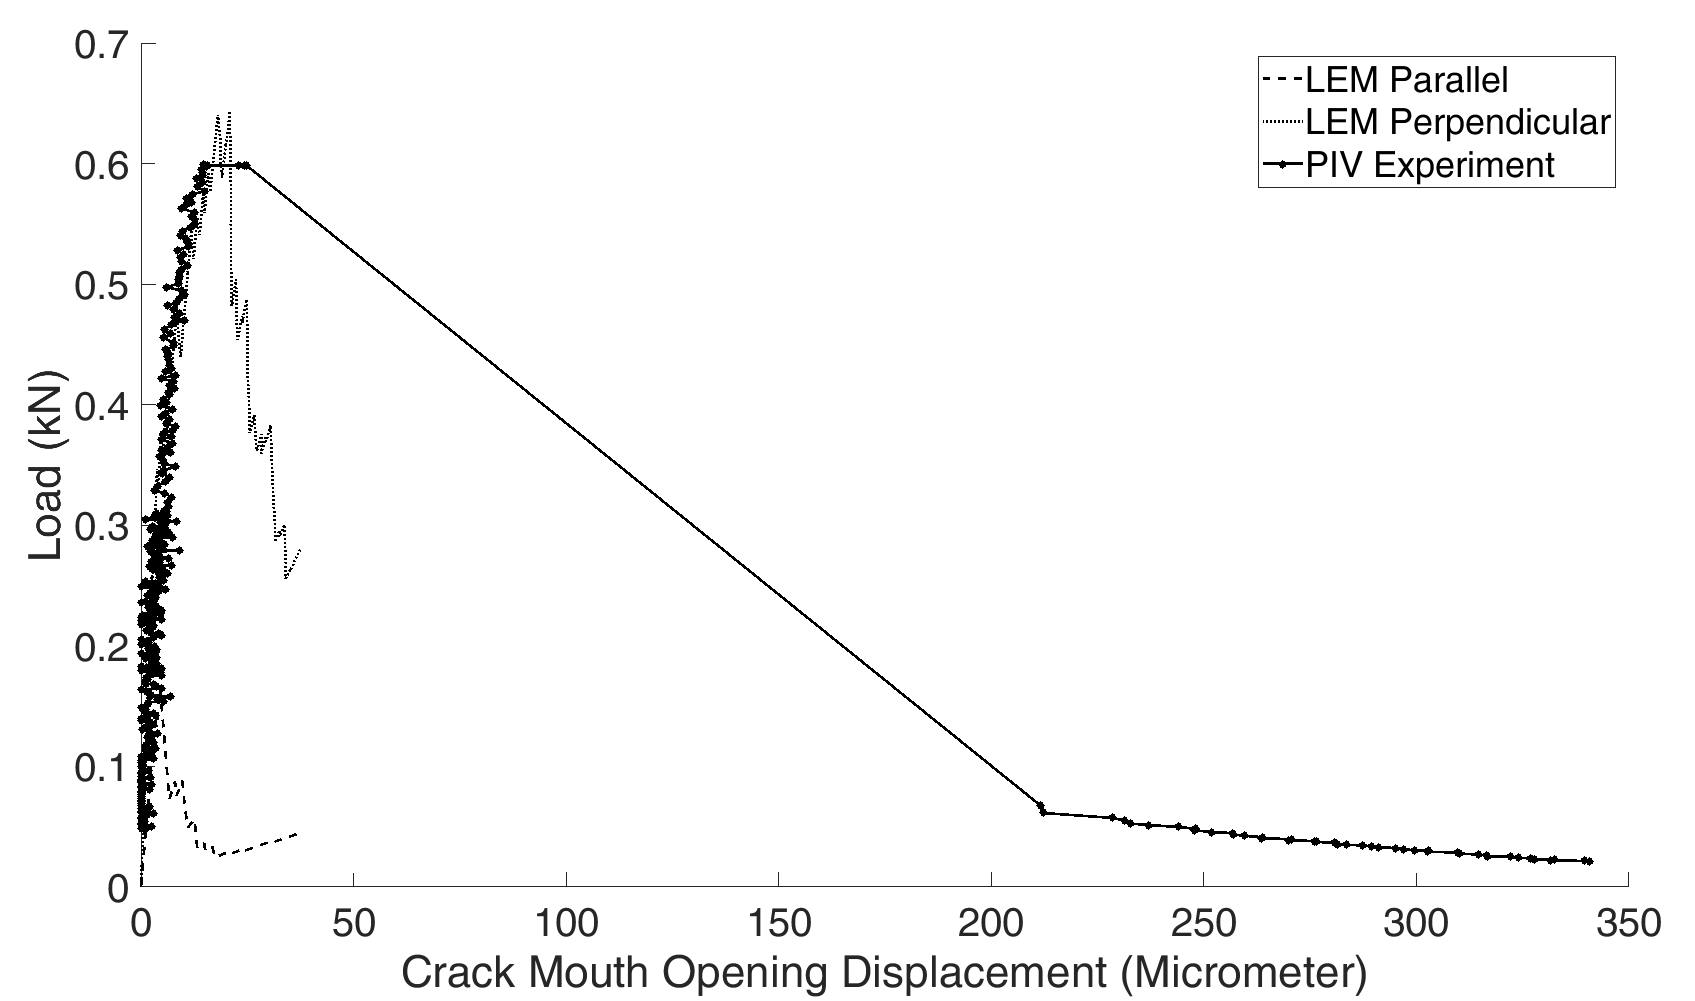
\includegraphics[width=0.75\textwidth]{figures/Amir_ME1_LEM_Claystone_Data.png}
\caption{The load vs. crack mouth opening displacement (CMOD) response of the Opalinus Clay}
\label{fig:Amir_ME1_LEM_Claystone_Data}
\end{figure}

\subsubsection*{UFZ}
The input files for OGS, which were used to simulate the three point bending test performed on the orthogonal and parallel laminations of Opalinus Clay samples, have been uploaded.
The files include the unstructured finite element mesh files in vtu format and OGS input files in xml format.
Also in the mesh files, the material properties are defined per element. 
Particularly for the orthogonal and the parallel Lamentations in the samples are represented through a contrast in the fracture toughness in the samples and can be found in the mesh files.
The load and crack mouth opening displacment computed from the simulations are shown in~\ref{fig:Keita_ME1_VPF_Claystone} as described in section \ref {sec:mex01b}.

\begin{figure}[!ht]
\centering
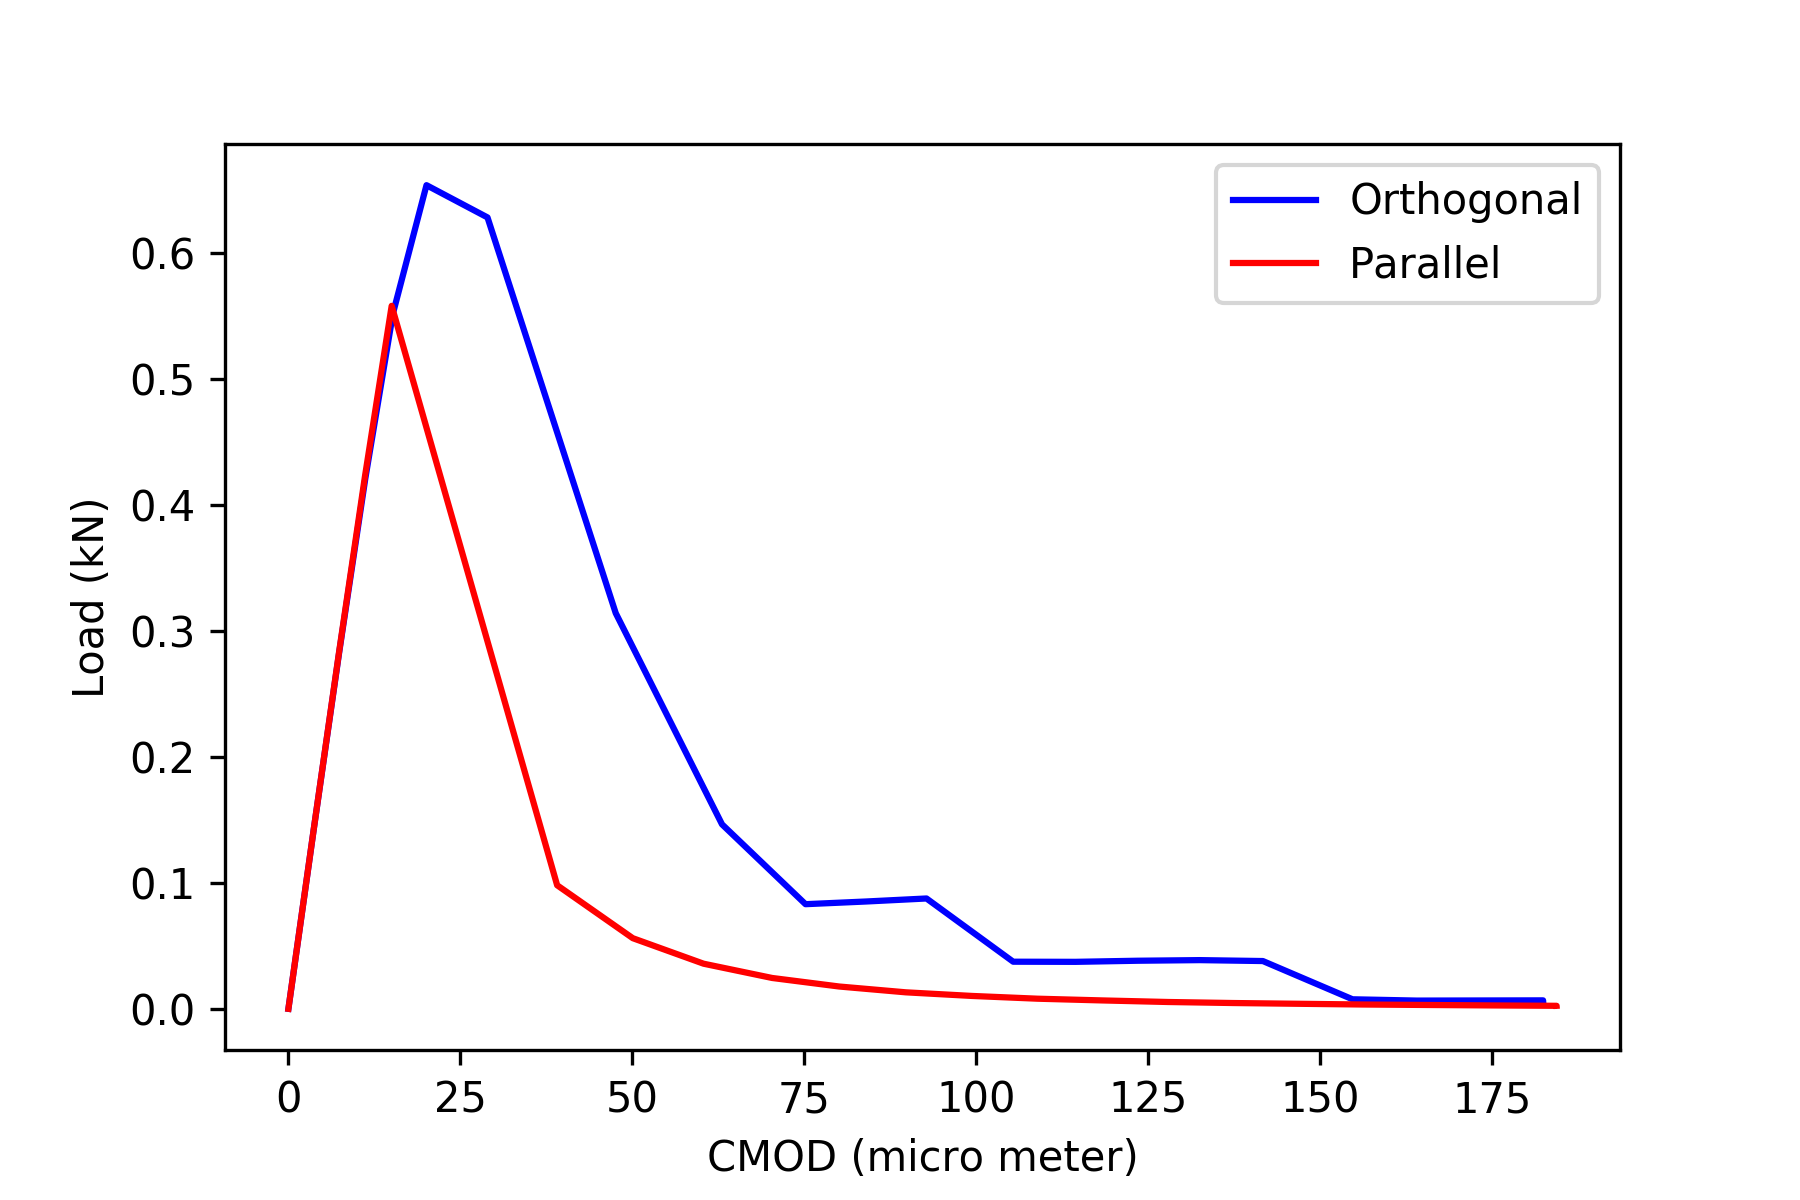
\includegraphics[width=0.75\textwidth]{figures/VPF_ME1_ex_NF_CMOD.png}
\caption{The load vs. crack mouth opening displacement (CMOD) response simulations for orthogonal and parallel lamination by VPF.}
\label{fig:Keita_ME1_VPF_Claystone}
\end{figure}

MEX 0-1b (UFZ) will be also provided as an OGS benchmark case at:\\
\small
\url{www.opengeosys.org/docs/benchmarks/phase-field/phasefield/pf_tpb_ani}
\normalsize

\clearpage
%---------------------------------------------------------
\subsubsection*{Meta Data Overview (according to Dublin Core)}
%---------------------------------------------------------

\begin{table}[!ht]
\caption{MEX 0-1b (CAU)}
\label{tab:dms-mex0-1b}
\small
\begin{tabular}{R{3.5cm}|L{7.5cm}}
\hline
%
Data label & GeomInt, MEX 0-1b, CAU, Bending fracture test, Opalinus Clay \\
URL (Experiments) & \url{https://nextcloud.ifg.uni-kiel.de/index.php/s/pJxp2eNEJb6PfiS} \\
URL (Numerics) & \url{https://nextcloud.ifg.uni-kiel.de/index.php/s/ZBFN2rSZ99kPY9M} \\
Subject  &  Bending fracture test, Opalinus Claye\\
Type of data  &  Experimental data, executable MATLAB P-file, input parameters\\
Subject  &  Bending fracture test, Opalinus Clay\\
Type of data  &  Experimental data, executable MATLAB P-file, input parameters\\
Data quality  &  Quality assured data \\
Status of data  &  Unprocessed data\\
Data format  & txt, xlsx, MATLAB executable P-file\\
Creators  &  Kiel University, Institute of Geomechanics and Geotechnics, Ludewig-Meyn-Stra\ss e 10, 24118, Kiel\\
Source/Origin & In-house code \\
Publisher  &  Kiel University, Institute of Geomechanics and Geotechnics, Ludewig-Meyn-Stra\ss e 10, 24118, Kiel \\
Rights holders &  Kiel University, Institute of Geomechanics and Geotechnics, Ludewig-Meyn-Stra\ss e 10, 24118, Kiel \\
Contributors &   Kiel University, Institute of Geomechanics and Geotechnics: Amir Shoarian Sattari, Frank Wuttke\\
Time/period of creation &  2018-2019\\
Language of the content &  English\\
Update policy &  Stored data is final\\
Access permissions & Full access\\
%
\hline
\end{tabular}
\end{table}

\begin{table}[!ht]
\caption{MEX 0-1b (UFZ)}
\label{tab:dms-mex0-1a}
\small
\begin{tabular}{R{3.5cm}|L{7.5cm}}
\hline
%
Data label & MEX 0-1b (UFZ) \\
URL & \url{www.opengeosys.org/docs/benchmarks/phase-field/phasefield/} \\ 
Subject  & Bending fracture test, Opalinus Clay \\
Type of data  & Data set (structured data in a defined format) \\
Data quality  & Quality assured data by benchmarking \\
Status of data  & Processed data \\
Data format  & OGS files \\
Creators  & Yoshioka, Keita  \\
Source/Origin & Open source \\
Publisher  & Helmholtz Centre for Environmental Research UFZ \\
Rights holders & Helmholtz Centre for Environmental Research UFZ \\
Contributors & Yoshioka, Keita \\
Time/period of creation & 2019-2020 \\
Language of content & English \\
Update policy & To be merged to OGS benchmarks (see below) \\
Access permissions & Free access \\
%
\hline
\end{tabular}
\end{table}

\clearpage
%------------------------------------------------------------------------
%%\subsection{MEX 1-1a:}
Data management for MEX 1-1a (see \ref{sec:mex05}).
%\todo[inline]{[CAU et al.]: Please add data management info for MEX 1-1a}

%%% Amir: This section should be removed. dms-mex11b already covers mex05. However, the experimental results from IfG is missing there


\begin{table}[!ht]
\caption{MEX 1-1a: Meta Data according to Dublin Core}
\label{tab:dms-mex1-1a}
\small
\begin{tabular}{R{3cm}|L{7cm}}
\hline
%
Data label &  \\
URI &  \\
Subject  &  \\
Type of data  &  \\
Dataquality  &  \\
Status of data  &  \\
Dataformat  & \\
Creators  &  \\
Source/Origin &  \\
Publisher  &  \\
Rights holders &  \\
Contributors &  \\
Time or Period of creation &  \\
Language of the content &  \\
Update policy &  \\
Access permissions &  \\
%
\hline
\end{tabular}
\end{table}
%%\clearpage
%------------------------------------------------------------------------
\subsection{MEX 1-1b: Swelling process, Salt Clay}

Data management for MEX 1-1b (see \ref{sec:mex05}).

\subsubsection*{CAU Kiel}
The required LEM code and the input variables for simulating the swelling process of the salt clay are uploaded to the IfG (Kiel) NextCloud server. The data is accessible through the following link:\\
\hyperlink{https://nextcloud.ifg.uni-kiel.de/index.php/s/JmZseQqrsbgWNqC}{https://nextcloud.ifg.uni-kiel.de/index.php/s/JmZseQqrsbgWNqC}\\

The uploaded protected MATLAB file in a *.p format requires a MATLAB version with a built-in Voronoi Tessellation and Delaunay Triangulation functions.Fig. \ref{fig:Amir_ME5_Lattice_Drying_Data} shows the change of hydraulic conductivity with applied linear strains as described in section \ref {sec:mex05}. 

\begin{figure}[!ht]
\centering
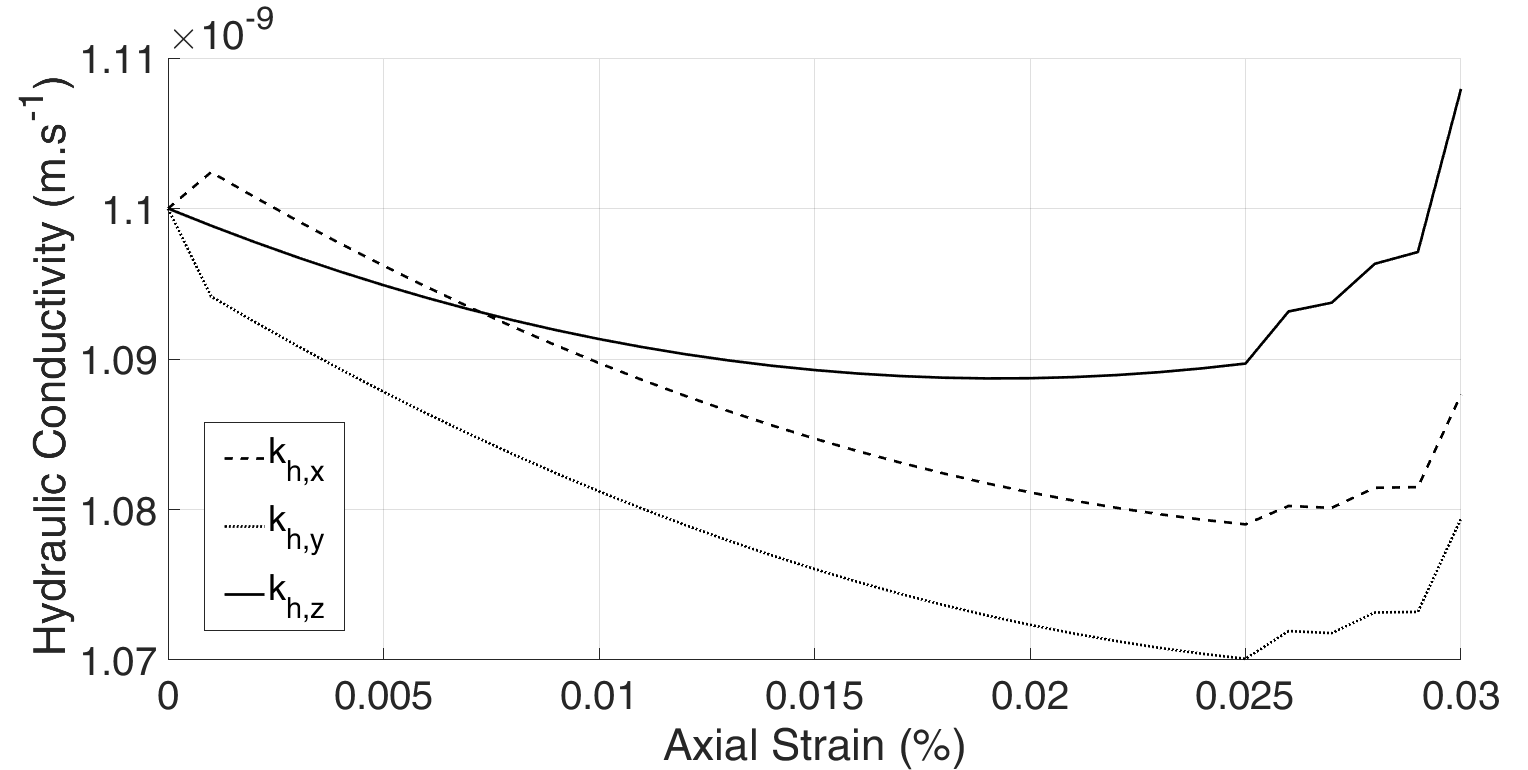
\includegraphics[width=0.75\textwidth]{figures/Amir_ME5_Lattice_Drying_Data.png}
\caption{The change of hydraulic conductivity with applied linear strains}
\label{fig:Amir_ME5_Lattice_Drying_Data}
\end{figure}

\begin{table}[!ht]
\caption{MEX 1-1b: Swelling process, salt clay}
\label{tab:dms-mex1-1b}
\small
\begin{tabular}{R{3cm}|L{7cm}}
\hline
%
Data label & GeomInt | CAU | Swelling process, salt clay\\
URI &  https://nextcloud.ifg.uni-kiel.de/index.php/s/JmZseQqrsbgWNqC (Numerics)\\
Subject  &  Swelling process, Salt Clay\\
Type of data  & executable MATLAB P-file, input parameters\\
Dataquality  &  quality assured data \\
Status of data  &  unprocessed data\\
Dataformat  & txt, MATLAB executable P-file\\
Creators  &  Kiel University, Institute of Geomechanics and Geotechnics, Ludewig-Meyn-Stra\ss e 10, 24118, Kiel\\
Source/Origin & In-house code \\
Publisher  &  Kiel University, Institute of Geomechanics and Geotechnics, Ludewig-Meyn-Stra\ss e 10, 24118, Kiel \\
Rights holders &  Kiel University, Institute of Geomechanics and Geotechnics, Ludewig-Meyn-Stra\ss e 10, 24118, Kiel \\
Contributors &   Kiel University, Institute of Geomechanics and Geotechnics: Amir Shoarian Sattari, Frank Wuttke\\
Time or Period of creation &  2019-2020\\
Language of the content &  English\\
Update policy &  stored data is final\\
Access permissions & full access\\
%
\hline
\end{tabular}
\end{table}
\clearpage
%------------------------------------------------------------------------
\subsection{MEX 1-2: Drying and wetting paths of the Opalinus Clay}

Participating institutions of MEX 1-2 (see section \ref{sec:mex06}): CAU, UFZ

\begin{table}[ht!]
\caption{MEX 1-2: Data overview}
\label{tab:dms-mex12-overview}
\small
\begin{tabular}{l|l|l|l|L{4.7cm}|l}
\hline
\rowcolor{cyan}
Type & Spec. & Owner & Access     & Comment                       & Stat \\ 
\hline
EXP  &   DRY    & CAU   & Open       & Output files are uploaded          & \cellcolor{green} \\
\hline \hline
MOD  & LEM   & CAU   & Open       & Executable MATLAB P-file               & \cellcolor{yellow} \\
     &       &       & Open       & Input files will be uploaded  & \cellcolor{yellow} \\
\hline
MOD  & FEM   & UFZ   & Open       & Branch to be merged into OGS  & \cellcolor{yellow} \\
     & VPF   &       & Open       & Input files available         & \cellcolor{yellow} \\
%
\hline
\end{tabular}
\end{table}
\normalsize

\subsubsection*{CAU Kiel}

The experimental results of the drying and wetting paths of the sandy Opalinus Clay are uploaded to the IfG (Kiel) NextCloud server. The data is accessible through the following link:\\
\url{https://nextcloud.ifg.uni-kiel.de/index.php/s/q6g25nWyWJKqzNB}

The experimental data (*.xlsx) of drying and wetting paths are uploaded to the server. The data includes the reading number, time (day), stain values in perpendicular and parallel orientations, weight of the sample and measured water content values. Fig. \ref{fig:Amir_ME6_Strain_Data} shows the change of the strains under the applied suction values.

\begin{figure}[!ht]
\centering
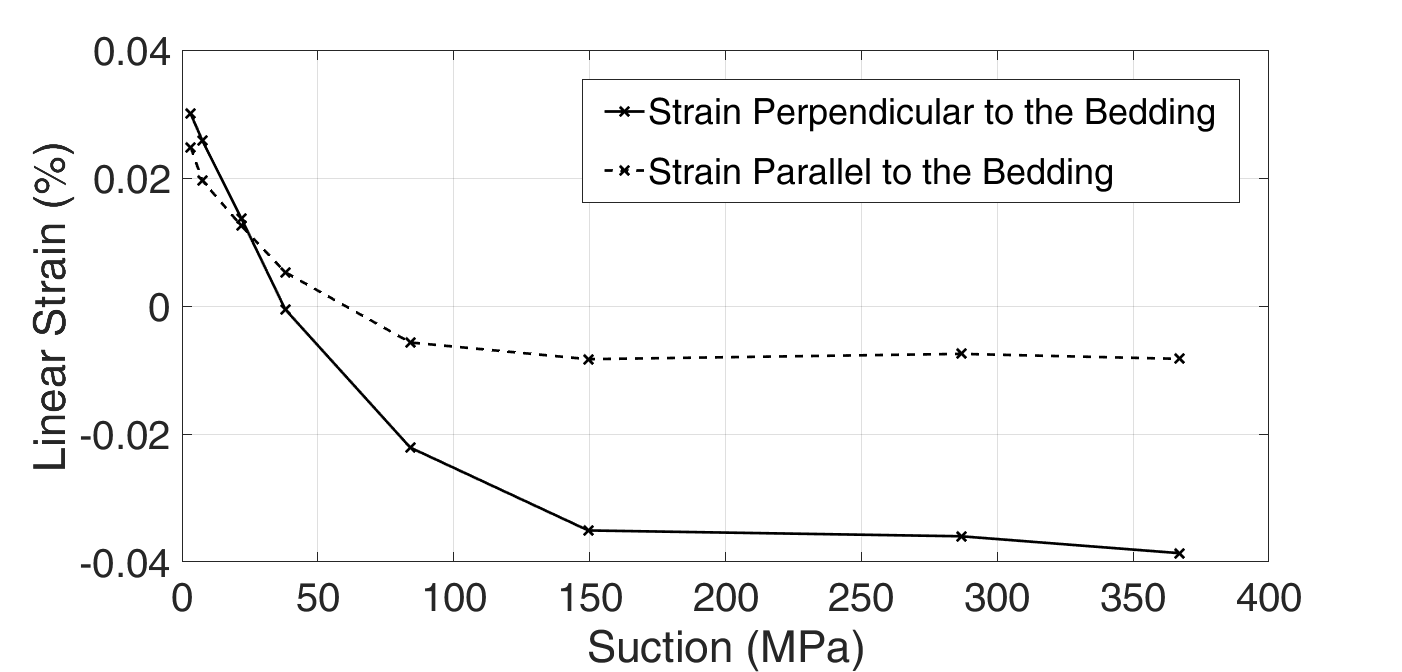
\includegraphics[width=0.75\textwidth]{figures/Amir_ME6_Strain_Data.png}
\caption{The suction vs. linear strains}
\label{fig:Amir_ME6_Strain_Data}
\end{figure}

The required LEM code and the input variables for simulating the drying and wetting paths of the sandy Opalinus Clay are uploaded to the IfG (Kiel) NextCloud server. The data is accessible through the following link:\\
\url{https://nextcloud.ifg.uni-kiel.de/index.php/s/fDNoPoXpXMqeAsK}

The uploaded protected MATLAB file in a *.p format requires a MATLAB version with a built-in Voronoi Tessellation and Delaunay Triangulation functions. Fig. \ref{fig:Amir_ME6_Lattice_Drying_Data} shows the change of hydraulic conductivity with applied linear strains as described in section \ref {sec:mex06}. 

\begin{figure}[!ht]
\centering
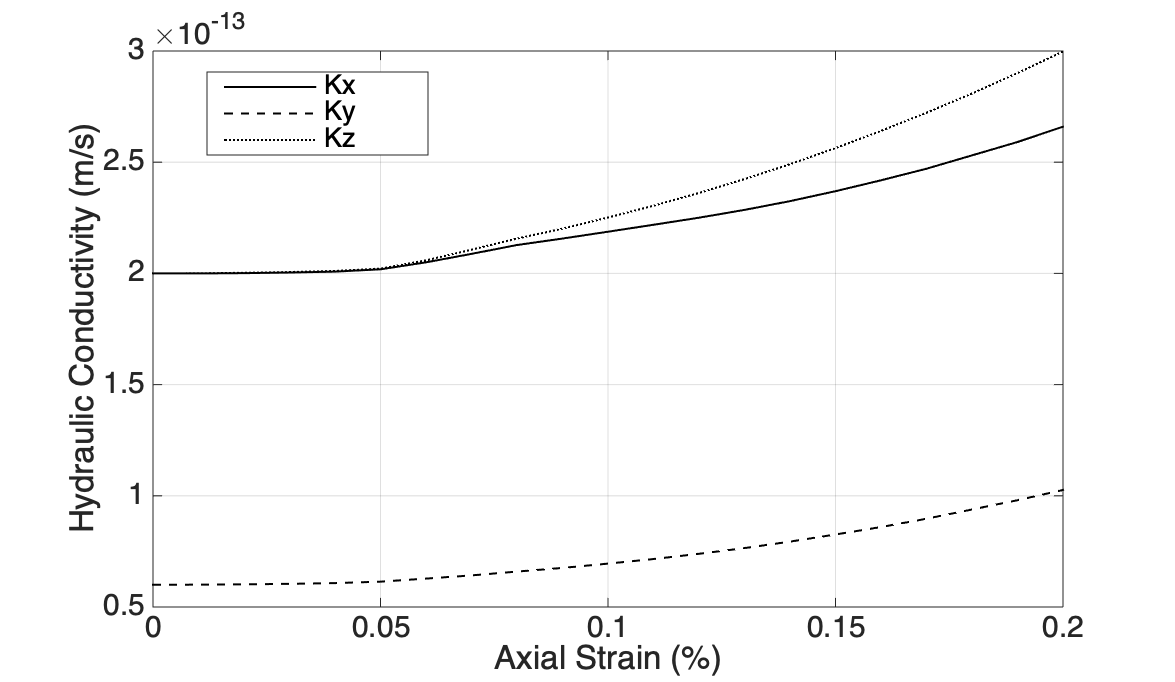
\includegraphics[width=0.6\textwidth]{figures/Amir_ME6_Lattice_Drying_Data.png}
\caption{The change of hydraulic conductivity with applied linear strains, Opalinus Clay}
\label{fig:Amir_ME6_Lattice_Drying_Data}
\end{figure}

%---------------------------------------------------------
\subsubsection*{Meta Data Overview (according to Dublin Core)}
%---------------------------------------------------------

\begin{table}[!ht]
\caption{MEX 1-2 (CAU)}
\label{tab:dms-mex1-2}
\small
\begin{tabular}{R{3.5cm}|L{7.5cm}}
\hline
%
Data label & GeomInt, MEX 1-2, CAU, drying and wetting paths, Opalinus Clay \\
URL (Experiments) & \url{https://nextcloud.ifg.uni-kiel.de/index.php/s/q6g25nWyWJKqzNB} \\
URL (Numerics) & \url{https://nextcloud.ifg.uni-kiel.de/index.php/s/fDNoPoXpXMqeAsK} \\
Subject  &  Drying and Wetting Paths (Opalinus Clay)\\
Type of data  & Experimental data, executable MATLAB P-file, input parameters\\
Data quality  &  Quality assured data \\
Status of data  &  Unprocessed data\\
Data format  & txt, xlsx, MATLAB executable P-file\\
Creators  &  Kiel University, Institute of Geomechanics and Geotechnics, Ludewig-Meyn-Stra\ss e 10, 24118, Kiel\\
Source/Origin & In-house code \\
Publisher  &  Kiel University, Institute of Geomechanics and Geotechnics, Ludewig-Meyn-Stra\ss e 10, 24118, Kiel \\
Rights holders &  Kiel University, Institute of Geomechanics and Geotechnics, Ludewig-Meyn-Stra\ss e 10, 24118, Kiel \\
Contributors &   Kiel University, Institute of Geomechanics and Geotechnics: Amir Shoarian Sattari, Frank Wuttke\\
Time/period of creation &  2018-2020\\
Language of the content &  English\\
Update policy &  Stored data is final\\
Access permissions & Full access\\
%
\hline
\end{tabular}
\end{table}
\clearpage
%------------------------------------------------------------------------
\subsection{MEX 1-4: CD/LP experiment (BGR)}

Data management for MEX 1-4 (see \ref{sec:mex10}).

Link to the data set at UFZ data investigation portal (Download only for project members):
\hyperlink{https://www.ufz.de/record/dmp/archive/7471/}{https://www.ufz.de/record/dmp/archive/7471/}

The data set contains all project files that are relevant to reproduce the simulation results described in Section \ref{sec:mex10} and its corresponding subsections. For every simulation run with OGS-6, the data set comprises a project file (\texttt{*.prj}), a geometry file (\texttt{*.gml}) and the computational mesh (\texttt{*.vtu}). For simulations run with OGS-5, the project is split into files for boundary conditions (\texttt{*.bc}), initial conditions (\texttt{*.ic}), fluid properties (\texttt{*.mfp}), material properties (\texttt{*.mmp}), solid properties (\texttt{*.msp}), numerical parameters (\texttt{*.num}), output parameters (\texttt{*.out}), process definitions (\texttt{*.pcs}), tabulated functional dependencies (\texttt{*.rfd}), source terms (\texttt{*.sc}), and output parameters (\texttt{*.out}). In addition, seperate files are provided for the geometry (\texttt{*.gli}) and the computational mesh (\texttt{*.msh}).

\begin{table}[!ht]
\caption{MEX 1-4: Meta Data according to Dublin Core}
\label{tab:dms-mex1-4}
\small
\begin{tabular}{R{3cm}|L{7cm}}
\hline
%
Data label &  \\
URI &  \\
Subject  &  \\
Type of data  &  \\
Dataquality  &  \\
Status of data  &  \\
Dataformat  & \\
Creators  &  \\
Source/Origin &  \\
Publisher  &  \\
Rights holders &  \\
Contributors &  \\
Time or Period of creation &  \\
Language of the content &  \\
Update policy &  \\
Access permissions &  \\
%
\hline
\end{tabular}
\end{table}
\clearpage
%------------------------------------------------------------------------
\subsection{MEX 2-1a: Pressure driven percolation in salt}

Participating institutions of MEX 2-1a (see section \ref{sec:mex02}): CAU, IfG, UFZ

\begin{table}[ht!]
\caption{MEX 2-1a: Data overview}
\label{tab:dms-mex21a-overview}
\small
\begin{tabular}{l|l|l|l|L{4.7cm}|l}
\hline
\rowcolor{cyan}
Type & Spec. & Owner & Access     & Comment                       & Stat \\ 
\hline 
EXP  & LIT   & \cite{Kamlot2009} & Restricted & Literature available online & \cellcolor{green} \\
\hline \hline
MOD  & LEM   & CAU   & License    & Executable MATLAB P-file      & \cellcolor{yellow} \\
     &       &       & Free       & I/O available                 & \cellcolor{yellow} \\
\hline
MOD  & FEM   & UFZ   & Open source & via OpenGeoSys portal        & \cellcolor{yellow} \\
     & VFP   &       & Free        & I/O available                & \cellcolor{green} \\
%
\hline
\end{tabular}
\end{table}
\normalsize

\subsubsection*{UFZ}

Link to the data set at UFZ data investigation portal (Download only for project members):
\url{https://www.ufz.de/record/dmp/archive/7706/}

The link contains two input decks for OGS-6 in which pressure driven percolation as described in MEX2 is simulated under different configurations of boundary loading.
The first case applies the boundary loading of 12 MPa, 21 MPa, and 8 MPa in x-, y-, and z-direction respectively. It is called ''case 1" and the corresponding OGS-6 input file is ''me2\_insitu\_case1.prj".
The second case is loaded with 4 MPa, 15 MPa, and 19 MPa in x-, y-, and z-direction respectively and the input file is named ''me2\_insitu\_case2.prj".
The remaining files are vtu files that describe the computing domain and the boundaries as shown in~\ref{fig:VPF_init}.

MEX 2-1a (UFZ) will be also provided as an OGS benchmark case at:\\
\small
\url{https://www.opengeosys.org/docs/benchmarks/phase-field/phasefield/}
\normalsize

\subsubsection*{CAU Kiel}

The required LEM code and the input variables of the percolation test on saltstone samples are uploaded to the IfG (Kiel) NextCloud server. The data is accessible through the following link:\\
\url{https://nextcloud.ifg.uni-kiel.de/index.php/s/9JZZcpS4S3JJT9S}

The uploaded protected MATLAB file in a *.p format requires a MATLAB version with a built-in Voronoi Tessellation and Delaunay Triangulation functions. The input variables are prepared in two files for two different stress configurations. Fig. \ref{fig:Amir_ME2_LEM_b_model_Fracture_Data} shows the frack surfaces under the percolation test as described in section \ref {sec:mex02}.

\begin{figure}[!ht]
\centering
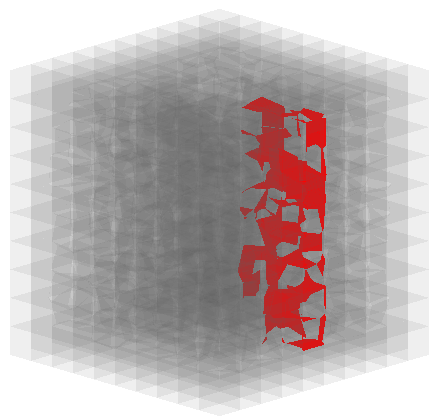
\includegraphics[width=0.7\textwidth]{figures/Amir_ME2_LEM_b_model_Fracture_Data.png}
\caption{The frack surfaces (red) under the percolation test, Saltstone}
\label{fig:Amir_ME2_LEM_b_model_Fracture_Data}
\end{figure}

%---------------------------------------------------------
\subsubsection*{Meta Data Overview (according to Dublin Core)}
%---------------------------------------------------------
\begin{table}[!ht]
\caption{MEX 2-1a (UFZ)}
\label{tab:dms-mex2-1a-ufz}
\small
\begin{tabular}{R{3.5cm}|L{7.5cm}}
\hline
%
Data label & MEX 0-1a (UFZ) \\
URL & \url{https://www.ufz.de/record/dmp/archive/7706/} \\ 
Subject  & Bending fracture test \\
Type of data  & Data set (structured data in a defined format) \\
Data quality  & Quality assured data by benchmarking \\
Status of data  & Processed data \\
Data format  & OGS files \\
Creators  & Yoshioka, Keita  \\
Source/Origin & Open source \\
Publisher  & Helmholtz Centre for Environmental Research UFZ \\
Rights holders & Helmholtz Centre for Environmental Research UFZ \\
Contributors & Yoshioka, Keita; Wang Wenqing \\
Time/period of creation & 2019-2020 \\
Language of content & English \\
Update policy & To be merged to OGS benchmarks (see below) \\
Access permissions & Free access \\
%
\hline
\end{tabular}
\end{table}

\begin{table}[!ht]
\caption{MEX 2-1a (CAU)}
\label{tab:dms-mex2-1a-cau}
\small
\begin{tabular}{R{3.5cm}|L{7.5cm}}
\hline
%
Data label & GeomInt | CAU | Percolation test, Saltstone\\
URI &  \url{https://nextcloud.ifg.uni-kiel.de/index.php/s/9JZZcpS4S3JJT9S} (Numerics)
\\
Subject  &  Percolation test (Saltstone)\\
Type of data  & Executable MATLAB P-file, input parameters\\
Dataquality  &  Quality assured data \\
Status of data  &  Unprocessed data\\
Dataformat  & txt, MATLAB executable P-file\\
Creators  &  Kiel University, Institute of Geomechanics and Geotechnics, Ludewig-Meyn-Stra\ss e 10, 24118, Kiel\\
Source/Origin & In-house code \\
Publisher  &  Kiel University, Institute of Geomechanics and Geotechnics, Ludewig-Meyn-Stra\ss e 10, 24118, Kiel \\
Rights holders &  Kiel University, Institute of Geomechanics and Geotechnics, Ludewig-Meyn-Stra\ss e 10, 24118, Kiel \\
Contributors &   Kiel University, Institute of Geomechanics and Geotechnics: Amir Shoarian Sattari, Frank Wuttke\\
Time/period of creation &  2018-2020\\
Language of the content &  English\\
Update policy &  Stored data is final\\
Access permissions & Full access\\
%
\hline
\end{tabular}
\end{table}
\clearpage
%------------------------------------------------------------------------
\subsection{MEX 2-1b: Pressure driven percolation, Opalinus claystone}

Participating institutions of MEX 2-1b (see section \ref{sec:mex2-1b}): CAU, UFZ

\subsubsection*{CAU Kiel}

The experimental results of the pressure driven percolation test on the cubic Opalinus claystone samples are uploaded to the IfG (Kiel) NextCloud server. The data is accessible through the following link:\\
\hyperlink{https://nextcloud.ifg.uni-kiel.de/index.php/s/EMdNkdF4PRKWCqa}{https://nextcloud.ifg.uni-kiel.de/index.php/s/EMdNkdF4PRKWCqa}\\

The experimental data (*.ASCII) of two different stress configurations (section \ref{sec:Percolation_Claystone_Exp}) are uploaded to the server. The data includes the time ($\Delta T=1s$), pump volume ($mL$), given oil pressure ($Bar$) and actual oil pressure in the system ($Bar$). Fig. \ref{fig:Amir_Percolation_Flow_a_Data}
illustrates an example of the plotted borehole pressure vs. flow volume for the $1^{st}$ stress configuration discussed in the section \ref{sec:mex2-1b}.

\begin{figure}[!ht]
\centering
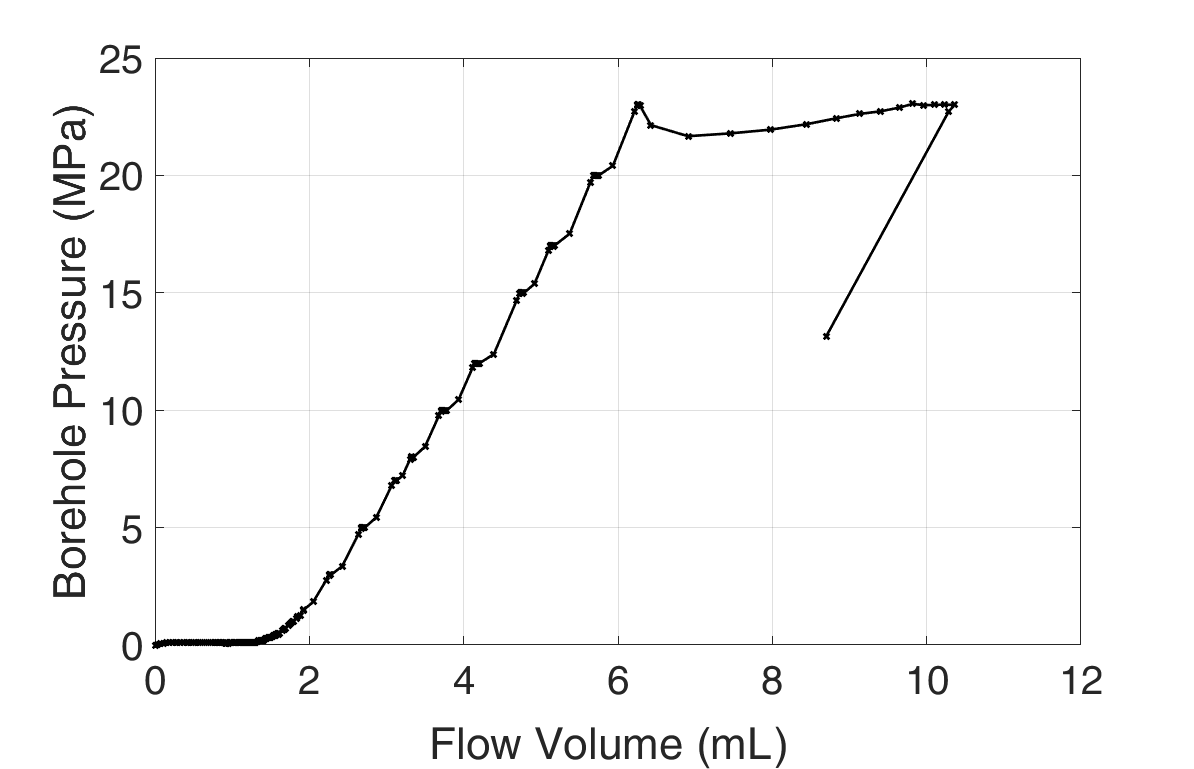
\includegraphics[width=0.75\textwidth]{figures/Amir_Percolation_Flow_a_Data.png}
\caption{The recorded results depicting the evolution of the borehole pressure vs. flow volume for the $1^{st}$ stress configuration}
\label{fig:Amir_Percolation_Flow_a_Data}
\end{figure}

The required LEM code and the input variables of the percolation test on Opalinus claystone samples are uploaded to the IfG (Kiel) NextCloud server. The data is accessible through the following link:\\
\hyperlink{https://nextcloud.ifg.uni-kiel.de/index.php/s/tFKKjxnSpgNG25b}{https://nextcloud.ifg.uni-kiel.de/index.php/s/tFKKjxnSpgNG25b}\\

The uploaded protected MATLAB file in a *.p format requires a MATLAB version with a built-in Voronoi Tessellation and Delaunay Triangulation functions. The input variables are prepared in two files for two different stress configurations. Fig. \ref{fig:Amir_ME2_B_Fracture_b_Data}
illustrates an example of the evolved frack surfaces for the $2^{nd}$ stress configuration discussed in the section  \ref{sec:mex2-1b}).

\begin{figure}[!ht]
\centering
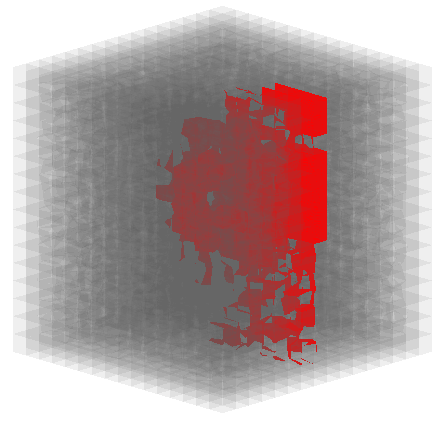
\includegraphics[width=4cm,height=4cm]{figures/Amir_ME2_B_Fracture_b_Data.png}
\caption{The frack surfaces (red) for the $2^{nd}$ stress configuration}
\label{fig:Amir_ME2_B_Fracture_b_Data}
\end{figure}

\begin{table}[!ht]
\caption{MEX 2-1b: Pressure driven percolation, Opalinus Claystone}
\label{tab:dms-mex2-1b}
\small
\begin{tabular}{R{3cm}|L{7cm}}
\hline
%
Data label & GeomInt | CAU | Percolation test, Opalinus claystone\\
URI &  https://nextcloud.ifg.uni-kiel.de/index.php/s/EMdNkdF4PRKWCqa (Experiments), https://nextcloud.ifg.uni-kiel.de/index.php/s/tFKKjxnSpgNG25b (Numerics)
\\
Subject  &  Percolation test, Opalinus claystone\\
Type of data  & Experimental data, Executable MATLAB P-file, Input parameters\\
Dataquality  &  quality assured data \\
Status of data  &  unprocessed data\\
Dataformat  & txt, ASCII, MATLAB executable P-file\\
Creators  &  Kiel University, Institute of Geomechanics and Geotechnics, Ludewig-Meyn-Stra\ss e 10, 24118, Kiel\\
Source/Origin & In-house code \\
Publisher  &  Kiel University, Institute of Geomechanics and Geotechnics, Ludewig-Meyn-Stra\ss e 10, 24118, Kiel \\
Rights holders &  Kiel University, Institute of Geomechanics and Geotechnics, Ludewig-Meyn-Stra\ss e 10, 24118, Kiel \\
Contributors &   Kiel University, Institute of Geomechanics and Geotechnics: Amir Shoarian Sattari, Frank Wuttke\\
Time or Period of creation &  2018-2020\\
Language of the content &  English\\
Update policy &  stored data is final\\
Access permissions & full access\\
%
\hline
\end{tabular}
\end{table}

\subsubsection*{UFZ}

\begin{table}[!ht]
\caption{MEX 2-1b (UFZ): Meta Data according to Dublin Core}
\label{tab:dms-mex2-1a}
\small
\begin{tabular}{R{3.5cm}|L{7.5cm}}
\hline
%
Data label & MEX 0-1a (UFZ) \\
URL & \colorbox{orange}{to be completed} \\ 
Subject  & Bending fracture test \\
Type of data  & Data set (structured data in a defined format) \\
Data quality  & Quality assured data by benchmarking \\
Status of data  & Processed data \\
Data format  & OGS files \\
Creators  & Yoshioka, Keita  \\
Source/Origin & Open source \\
Publisher  & Helmholtz Centre for Environmental Research UFZ \\
Rights holders & Helmholtz Centre for Environmental Research UFZ \\
Contributors & Yoshioka, Keita \\
Time/period of creation & 2019-2020 \\
Language of content & English \\
Update policy & To be merged to OGS benchmarks (see below) \\
Access permissions & Free access \\
%
\hline
\end{tabular}
\end{table}

MEX 2-1b (UFZ) will be also provided as an OGS benchmark case at:\\
\small
\url{https://www.opengeosys.org/docs/benchmarks/phase-field/phasefield/}
\normalsize
\clearpage
%------------------------------------------------------------------------
\subsection{MEX 2-2: Closure and healing of cracks (IfG)}

Data management for MEX 2-2 (see \ref{sec:mex03}).

The measured gas flow is converted into permeabilities, which are stored as time series in an Excel file. For each of the three experiment there are two columns. The first contains the time in hours since the start of the experiment, the second contains the permeability. 

\begin{figure}[!ht]
\centering
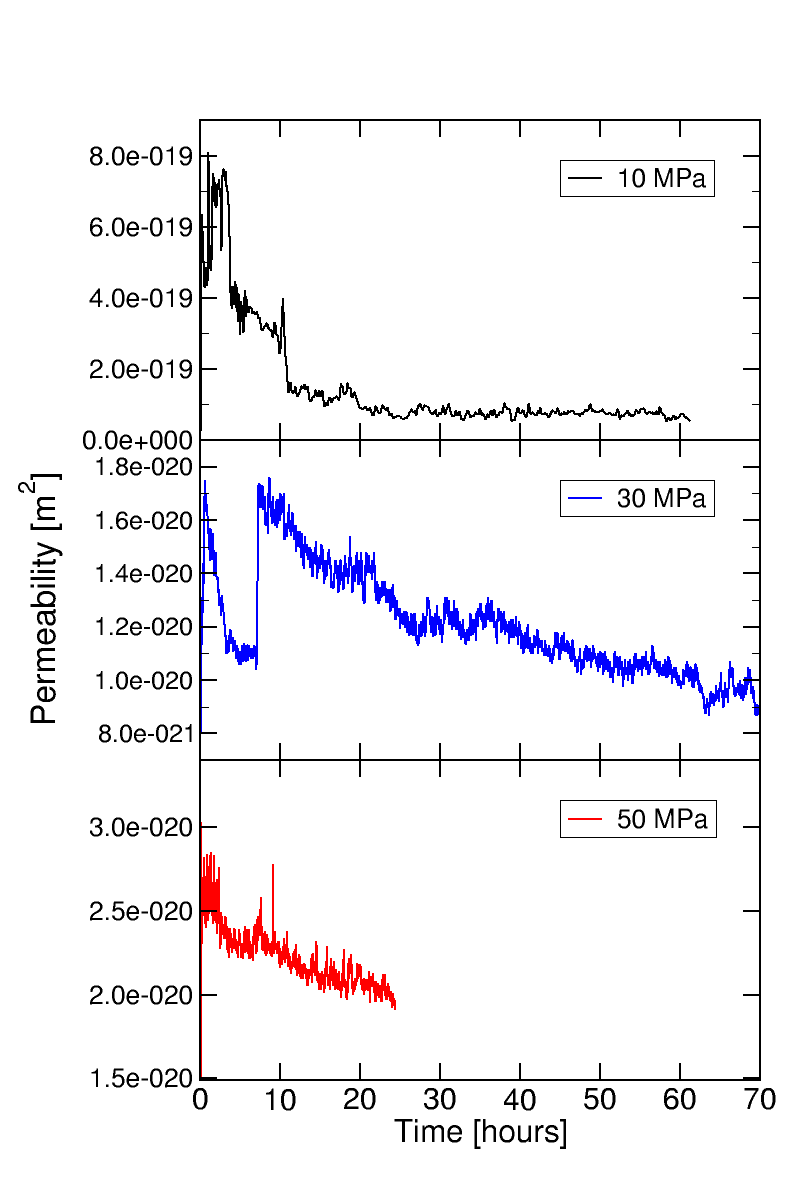
\includegraphics[width=0.75\textwidth]{figures/mex3-perme-time-comparison.png}
\caption{Graphical Representation of data.}
\label{fig:ME3-perme-exp-dmp}
\end{figure}

\begin{table}[!ht]
\caption{MEX 2-2: Meta Data according to Dublin Core}
\label{tab:dms-mex2-2}
\small
\begin{tabular}{R{3cm}|L{7cm}}
\hline
%
Data label &  \\
URI &  \\
Subject  &  \\
Type of data  &  \\
Dataquality  &  \\
Status of data  &  \\
Dataformat  & \\
Creators  &  \\
Source/Origin &  \\
Publisher  &  \\
Rights holders &  \\
Contributors &  \\
Time or Period of creation &  \\
Language of the content &  \\
Update policy &  \\
Access permissions &  \\
%
\hline
\end{tabular}
\end{table}
\clearpage
%------------------------------------------------------------------------
\subsection{MEX 2-3: Effect of compressibility on pressure driven percolation}

Data management for MEX 2-3 (see \ref{sec:mex04}).

\subsubsection*{CAU Kiel}

The required LEM code and the input variables for simulating the effect of compressibility are uploaded to the IfG (Kiel) NextCloud server. The data is accessible through the following link:\\
\hyperlink{https://nextcloud.ifg.uni-kiel.de/index.php/s/6Mfg3P4PyKNN6By}{https://nextcloud.ifg.uni-kiel.de/index.php/s/6Mfg3P4PyKNN6By}\\

The uploaded protected MATLAB file in a *.p format requires a MATLAB version with a built-in Voronoi Tessellation and Delaunay Triangulation functions. The input variables are prepared in two different files for the simulation of the pressure drop in gas and brine reservoirs. Fig. \ref{fig:Amir_ME4_Pressure_Data} shows the differences between the pressure drop in gas and brine reservoirs.

\begin{figure}[!ht]
\centering
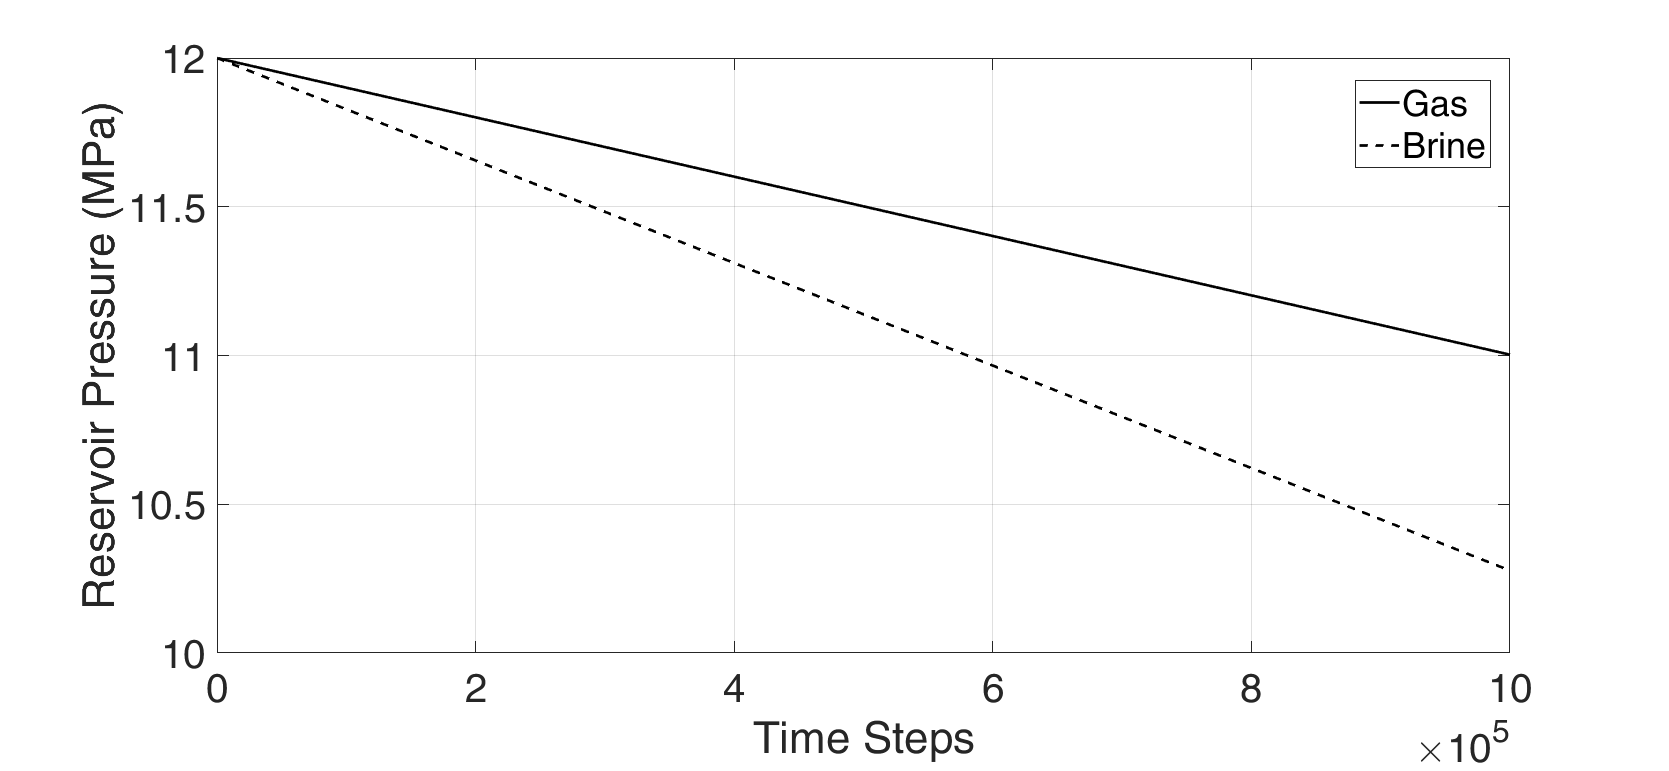
\includegraphics[width=8cm,height=5cm]{figures/Amir_ME4_Pressure_Data.png}
\caption{The comparison between the pressure drop in gas and brine reservoirs}
\label{fig:Amir_ME4_Pressure_Data}
\end{figure}


\begin{table}[!ht]
\caption{MEX 2-3: Effect of compressibility}
\label{tab:dms-mex2-3}
\small
\begin{tabular}{R{3cm}|L{7cm}}
\hline
%
Data label & GeomInt | CAU | Percolation test, effect of compressibility\\
URI &  https://nextcloud.ifg.uni-kiel.de/index.php/s/6Mfg3P4PyKNN6By (Numerics)
\\
Subject  &  Effect of compressibility\\
Type of data  & Executable MATLAB P-file, Input parameters\\
Dataquality  &  quality assured data \\
Status of data  &  unprocessed data\\
Dataformat  & txt, MATLAB executable P-file\\
Creators  &  Kiel University, Institute of Geomechanics and Geotechnics, Ludewig-Meyn-Stra\ss e 10, 24118, Kiel\\
Source/Origin & In-house code \\
Publisher  &  Kiel University, Institute of Geomechanics and Geotechnics, Ludewig-Meyn-Stra\ss e 10, 24118, Kiel \\
Rights holders &  Kiel University, Institute of Geomechanics and Geotechnics, Ludewig-Meyn-Stra\ss e 10, 24118, Kiel \\
Contributors &   Kiel University, Institute of Geomechanics and Geotechnics: Amir Shoarian Sattari, Frank Wuttke\\
Time or Period of creation &  2019-2020\\
Language of the content &  English\\
Update policy &  stored data is final\\
Access permissions & full access\\
%
\hline
\end{tabular}
\end{table}


\todo[inline]{[IfG et al.]: Please add data management info for MEX 2-3}

\begin{table}[!ht]
\caption{MEX 2-3: Meta Data according to Dublin Core}
\label{tab:dms-mex2-3}
\small
\begin{tabular}{R{3cm}|L{7cm}}
\hline
%
Data label &  \\
URI &  \\
Subject  &  \\
Type of data  &  \\
Dataquality  &  \\
Status of data  &  \\
Dataformat  & \\
Creators  &  \\
Source/Origin &  \\
Publisher  &  \\
Rights holders &  \\
Contributors &  \\
Time or Period of creation &  \\
Language of the content &  \\
Update policy &  \\
Access permissions &  \\
%
\hline
\end{tabular}
\end{table}
\clearpage
%------------------------------------------------------------------------
\subsection{MEX 2-4: Large wellbore test (Springen)}

Participating institutions of MEX 2-4 (see section \ref{sec:mex11}): IfG

\begin{table}[ht!]
\caption{MEX 2-4: Data overview}
\label{tab:dms-mex24-overview}
\small
\begin{tabular}{l|l|l|l|L{4.7cm}|l}
\hline
\rowcolor{cyan}
Type & Spec. & Owner & Access     & Comment                       & Stat \\ 
\hline 
EXP  & URL   & IfG   & Restricted & Available on demand           & \cellcolor{green} \\
\hline \hline
MOD  & DEM   & IfG   & License    & Commercial software           & \cellcolor{green} \\
     &       &       & Restricted & I/O available on demand       & \cellcolor{green} \\
\hline
\end{tabular}
\end{table}
\normalsize

%---------------------------------------------------------
\subsubsection*{Meta Data Overview (according to Dublin Core)}
%---------------------------------------------------------

\begin{table}[!ht]
\caption{MEX 2-4 (IfG)}
\label{tab:dms-mex2-4}
\small
\begin{tabular}{R{3cm}|L{7cm}}
\hline
%
Data label &  \\
URL &  \\
Subject  &  \\
Type of data  &  \\
Data quality  &  \\
Status of data  &  \\
Data format  & \\
Creators  &  \\
Source/Origin &  \\
Publisher  &  \\
Rights holders &  \\
Contributors &  \\
Time/period of creation &  \\
Language of the content &  \\
Update policy &  \\
Access permissions &  \\
%
\hline
\end{tabular}
\end{table}
\clearpage
%------------------------------------------------------------------------
\subsection{MEX 3-1: CNL direct shear test data (TUBAF)}\label{DataManMex3-1CNL}\index{Constant Normal Load (CNL) experiment}

Data management for MEX 3-1 (see \ref{sec:mex07}).

Link to the data set at UFZ data investigation portal: \url{https://www.ufz.de/record/dmp/archive/7925/}

The CNL data set contains four text files. One text file with the rock properties of the used granite (see Tab. \ref{table:MEX7_rockParam}). Two files with the scan data of the two surfaces. One point cloud can be seen in Fig. \ref{fig:DataCNLGranitePointCloud}. The last file contains the laboratory data. In Fig. \ref{fig:DataCNLGraniteLab} the results for the four shear stress levels can be seen.

\begin{figure}[!ht]
\begin{center}
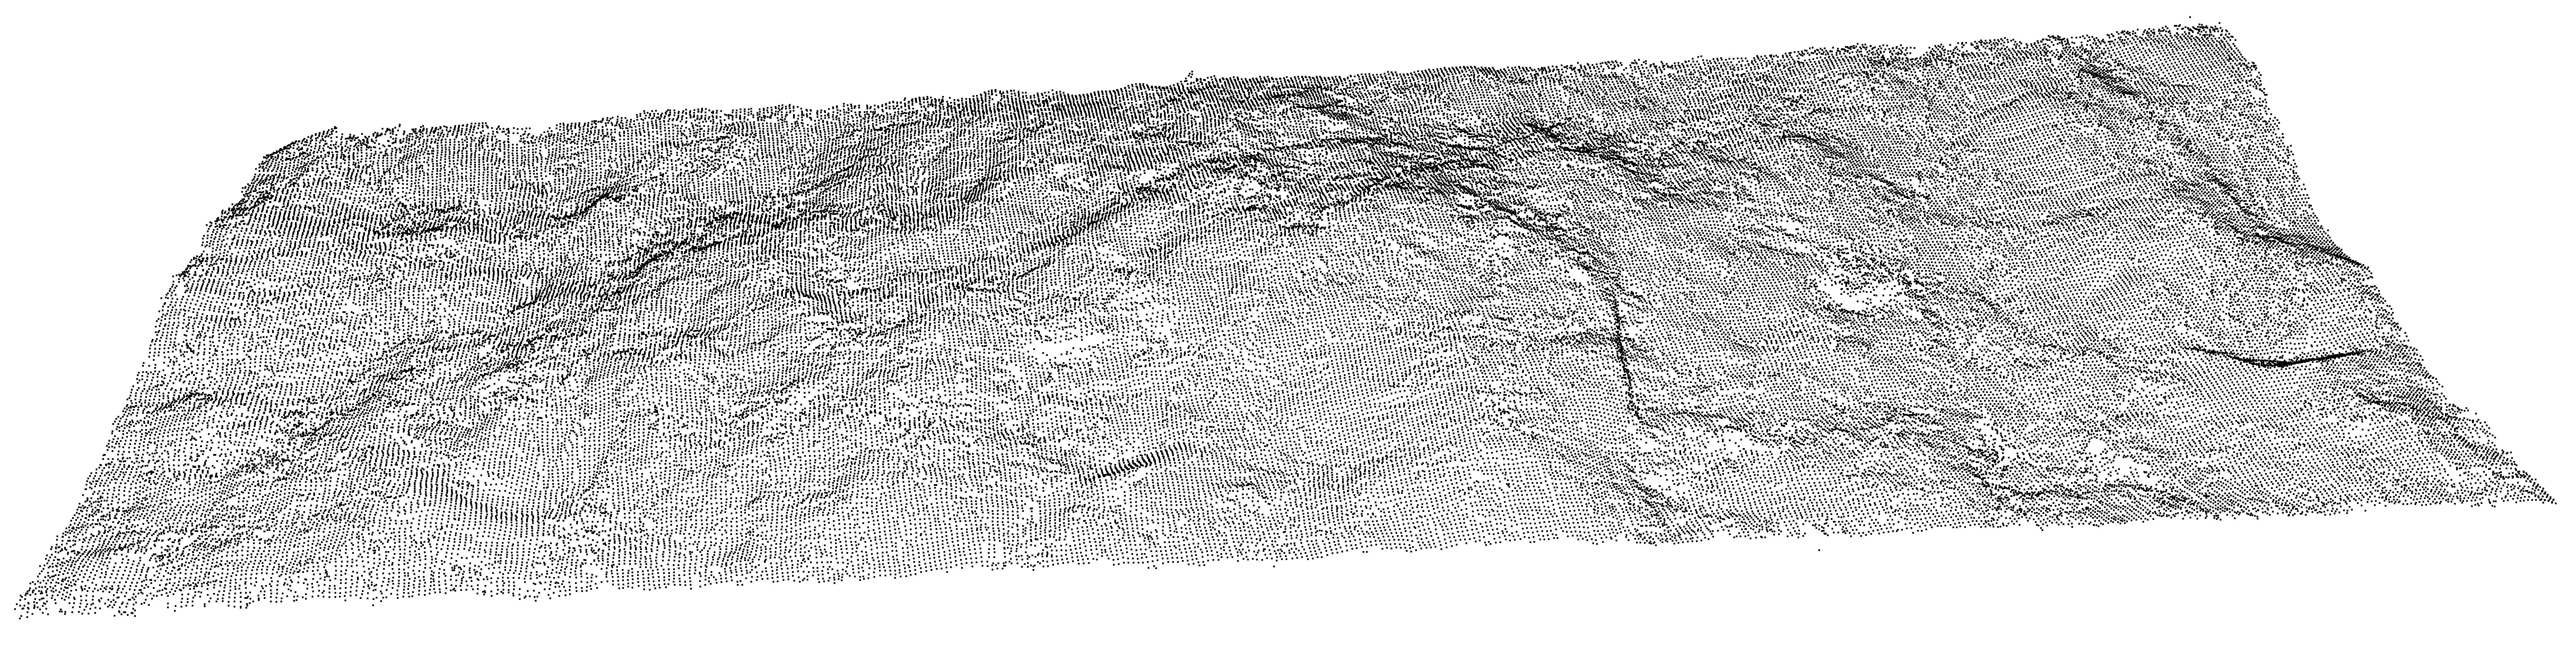
\includegraphics[width=0.75\textwidth]{./figures/MEX7_Point_cloud.png}
\end{center}
\caption{Point cloud representing the surface of a granite sample from Saxony. The size is 65 mm by 170 mm and the cloud contains approx. 98000 points.}
\label{fig:DataCNLGranitePointCloud}
\end{figure}

\begin{figure}[!ht]
\begin{tabular}{cc}
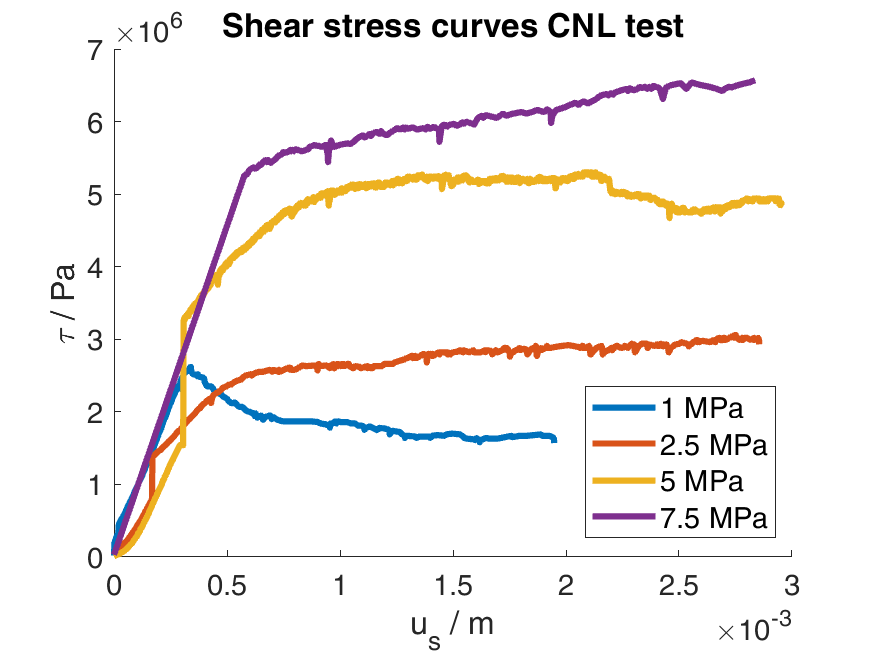
\includegraphics[width=0.45\textwidth]{./figures/CNLShearCurvesAll.png}     
& 
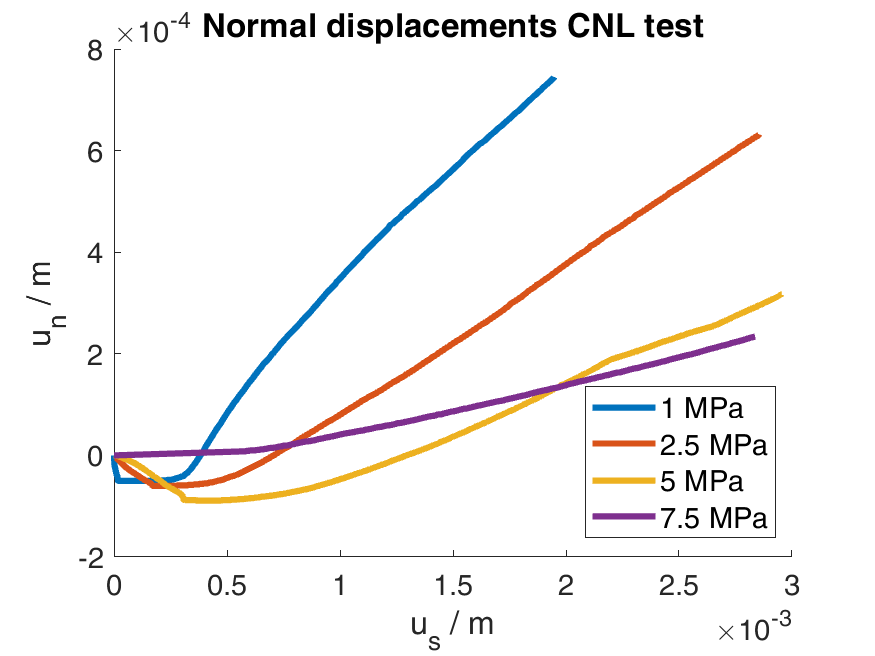
\includegraphics[width=0.45\textwidth]{./figures/CNLDilatationAll.png} 
\end{tabular}
\caption{CNL test results}
\label{fig:DataCNLGraniteLab}
\end{figure}

\begin{table}[!ht]
\caption{MEX 3-1: Meta Data according to Dublin Core}
\label{tab:dms-mex3-1}
\small
\begin{tabular}{R{3cm}|L{7cm}}
\hline
%\rowcolor{Cyan}
%
Data label & GeomInt | TUBAF | Data Set CNL \\
URI & http://www.ufz.de/record/dmp/archive/7925 \\
Subject  & Crystalline rock, direct shear test \\
Type of data  & collection of various data \\
Dataquality  & quality assured data \\
Status of data  & processed data \\
Dataformat  & txt, jpg, png \\
Creators  & TU Freiberg, Institut für Geotechnik, Gustav-Zeuner-Str. 1, 09599 Freiberg \\
Source/Origin  & Rock mechanical laboratory \\
Publisher  & TU Freiberg, Institut für Geotechnik, Gustav-Zeuner-Str. 1, 09599 Freiberg \\
Rights holders  & TU Freiberg, Institut für Geotechnik, Gustav-Zeuner-Str. 1, 09599 Freiberg \\
Contributors  & TU Freiberg, Institut für Geotechnik, Thomas Fr\"uhwirt and Daniel P\"otschke \\
Time or Period of creation  & 2018 - 2019 \\
Language of the content & English \\
Update policy  & stored data will not be extended \\
Access permissions  & limited access \\
%
\hline
\end{tabular}
\end{table}
\clearpage
%------------------------------------------------------------------------
%-------------------------------------------------------------------------------------------------
\subsection{MEX 3-2: CNS test}
\label{DataManMex3-2CNS}
\index{Constant Normal Stiffness (CNS) experiment}

Participating institutions of MEX 3-2 (see section \ref{sec:mex08}): TUBAF

\begin{table}[ht!]
\caption{MEX 3-2: Data overview}
\label{tab:dms-mex32-overview}
\small
\begin{tabular}{l|l|l|l|L{4.7cm}}
\hline
\rowcolor{cyan}
Type & Spec. & Owner & Access     & Comment                 \\ 
\hline 
EXP  & LAB   & TUBAF & Limited    & Available, UFZ-DMP      \\
\hline \hline
MOD  & FFS   & TUBAF & Open source & Available via GitHub   \\
     &       &       & Free       & I/O available           \\
\hline
\end{tabular}
\end{table}
\normalsize

Link to the data set at UFZ data management portal (DMP): \\ \url{https://www.ufz.de/record/dmp/archive/7924/}

The data set of the CNS test contains a file with the rock properties of the used basalt (see Tab. \ref{table:MEX7_rockParam}), two files with the scan data of the two surfaces. One point cloud can be seen in Fig. \ref{fig:DataCNSBasaltPointCloud}. The results of the laboratory tests are available as ASCII files and the shear curves and the dilatation are visualized in Fig. \ref{fig:DataCNSBasaltLab}. Additionally three photos of the basalt surface before, after the first and after the fourth shear test are included. 

\begin{figure}[!ht]
\begin{center}
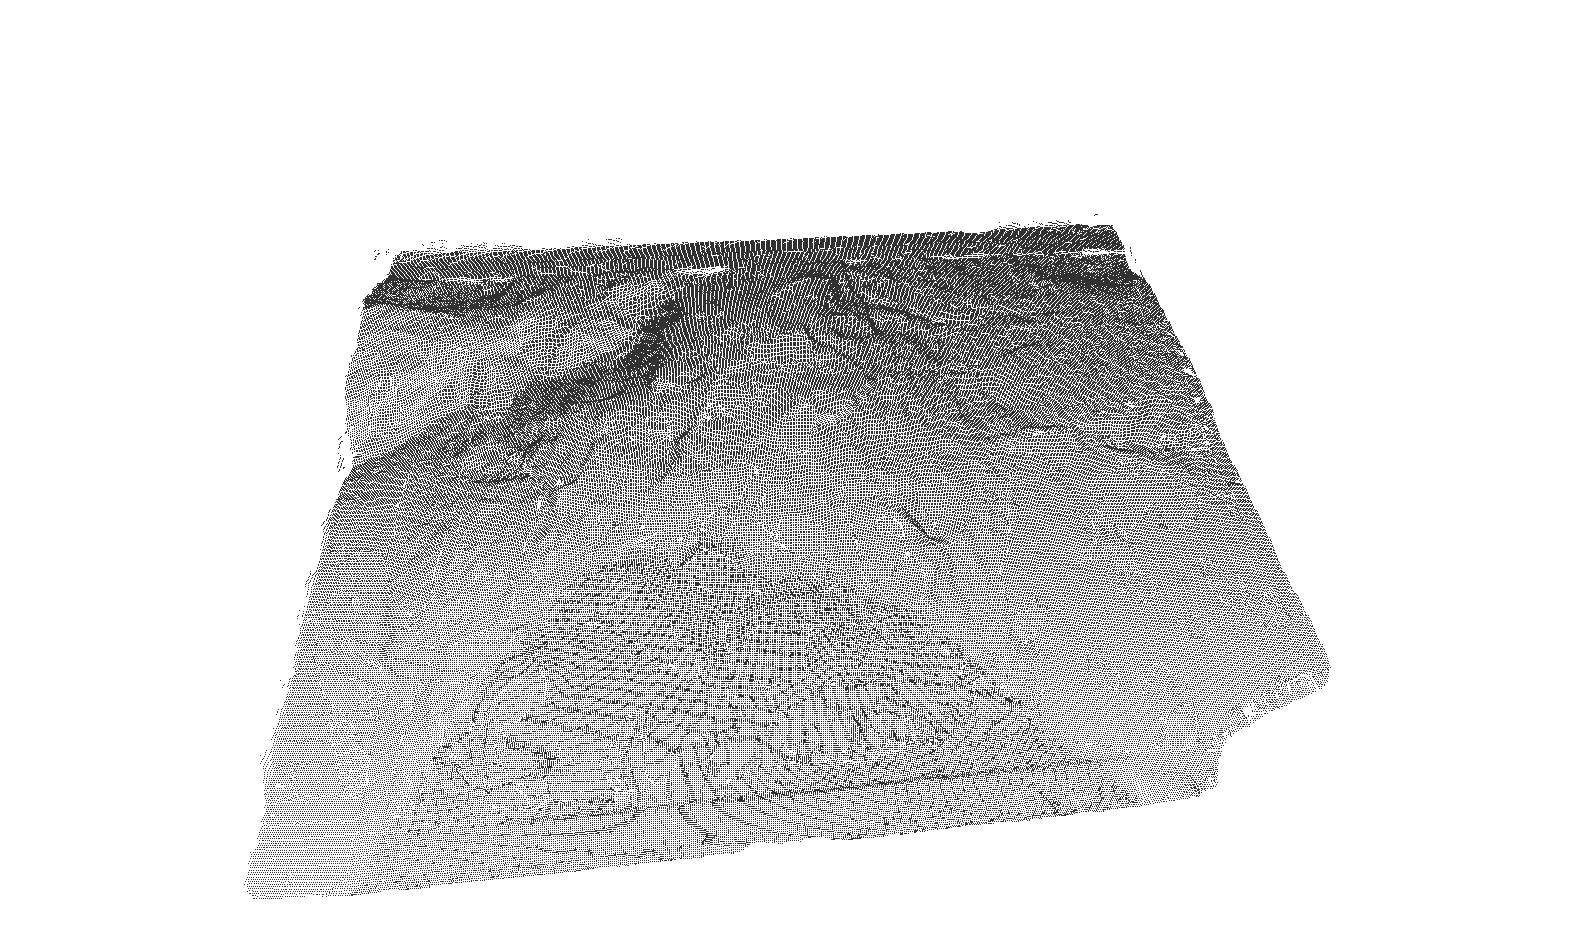
\includegraphics[width=0.6\textwidth]{./figures/MEX3-2PointCloud.png}
\end{center}
\caption{Point cloud representing the surface of a basalt sample from Thuringia. The size is 196 mm by 149 mm and the cloud contains approx. 252000 points.}
\label{fig:DataCNSBasaltPointCloud}
\end{figure}

\begin{figure}[!ht]
\begin{tabular}{cc}
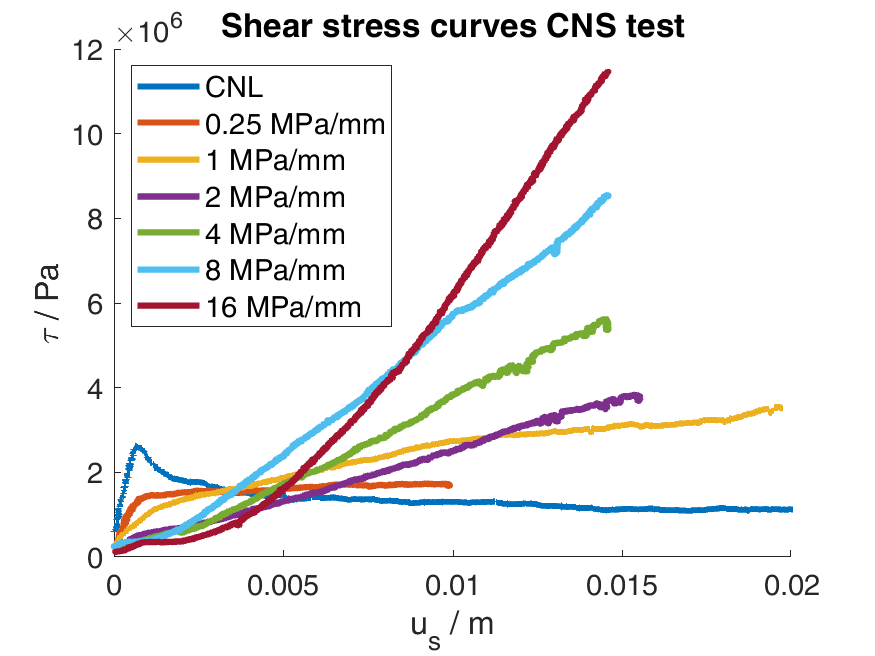
\includegraphics[width=0.45\textwidth]{./figures/CNSShearCurvesAll.png}     
& 
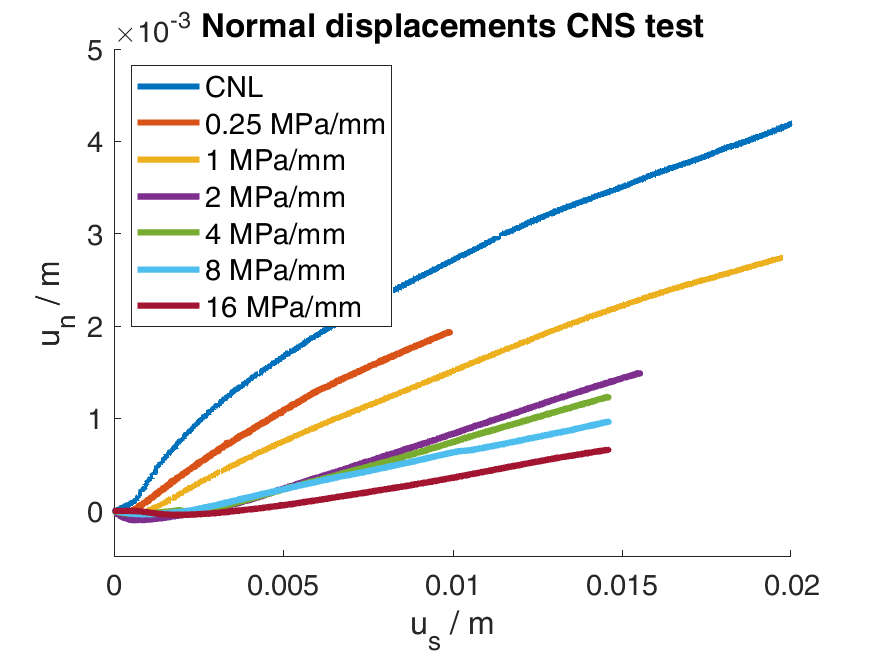
\includegraphics[width=0.45\textwidth]{./figures/CNSDilatationAll.png} 
\end{tabular}
\caption{CNS test results}
\label{fig:DataCNSBasaltLab}
\end{figure}

%---------------------------------------------------------
\subsubsection*{Meta Data Overview (according to Dublin Core)}
%---------------------------------------------------------

\begin{table}[!ht]
\caption{MEX 3-2 (TUBAF)}
\label{tab:dms-mex3-2}
\small
\begin{tabular}{R{3cm}|L{7cm}}
\hline
%
Data label & GeomInt, MEX 3-2, TUBAF, Data Set CNS \\
URI &  \url{http://www.ufz.de/record/dmp/archive/7924} \\
Subject  & Crystalline rock, direct shear test \\
Type of data  & collection of various data \\
Dataquality  & quality assured data \\
Status of data  & processed data \\
Dataformat  & txt, jpg, png \\
Creators  & TU Freiberg, Institut für Geotechnik, Gustav-Zeuner-Str. 1, 09599 Freiberg \\
Source/Origin  & Rock mechanical laboratory \\
Publisher  & TU Freiberg, Institut für Geotechnik, Gustav-Zeuner-Str. 1, 09599 Freiberg \\
Rights holders  & TU Freiberg, Institut für Geotechnik, Gustav-Zeuner-Str. 1, 09599 Freiberg \\
Contributors  & TU Freiberg, Institut für Geotechnik, Thomas Fr\"uhwirt and Daniel P\"otschke \\
Time/period of creation  & 2018 - 2019 \\
Language of the content & English \\
Update policy  & Stored data will not be extended \\
Access permissions  & Limited access \\
%
\hline
\end{tabular}
\end{table}
\clearpage
%------------------------------------------------------------------------
%-------------------------------------------------------------------------------------------------
\subsection{MEX 3-3: Inverse Analysis of Reiche Zeche Field Data}

Data management for model used throughout MEX 3-3 (see \ref{sec:mex09}).

Link to the data set stored at the Gitlab server located at the Institute of Applied Mechanics, University of Stuttgart:\\
\hyperlink{https://galilei.isr.uni-stuttgart.de/gitlab/schmidt/geomint}{https://galilei.isr.uni-stuttgart.de/gitlab/schmidt/geomint}\\
\begin{figure}[!ht]
\begin{center}
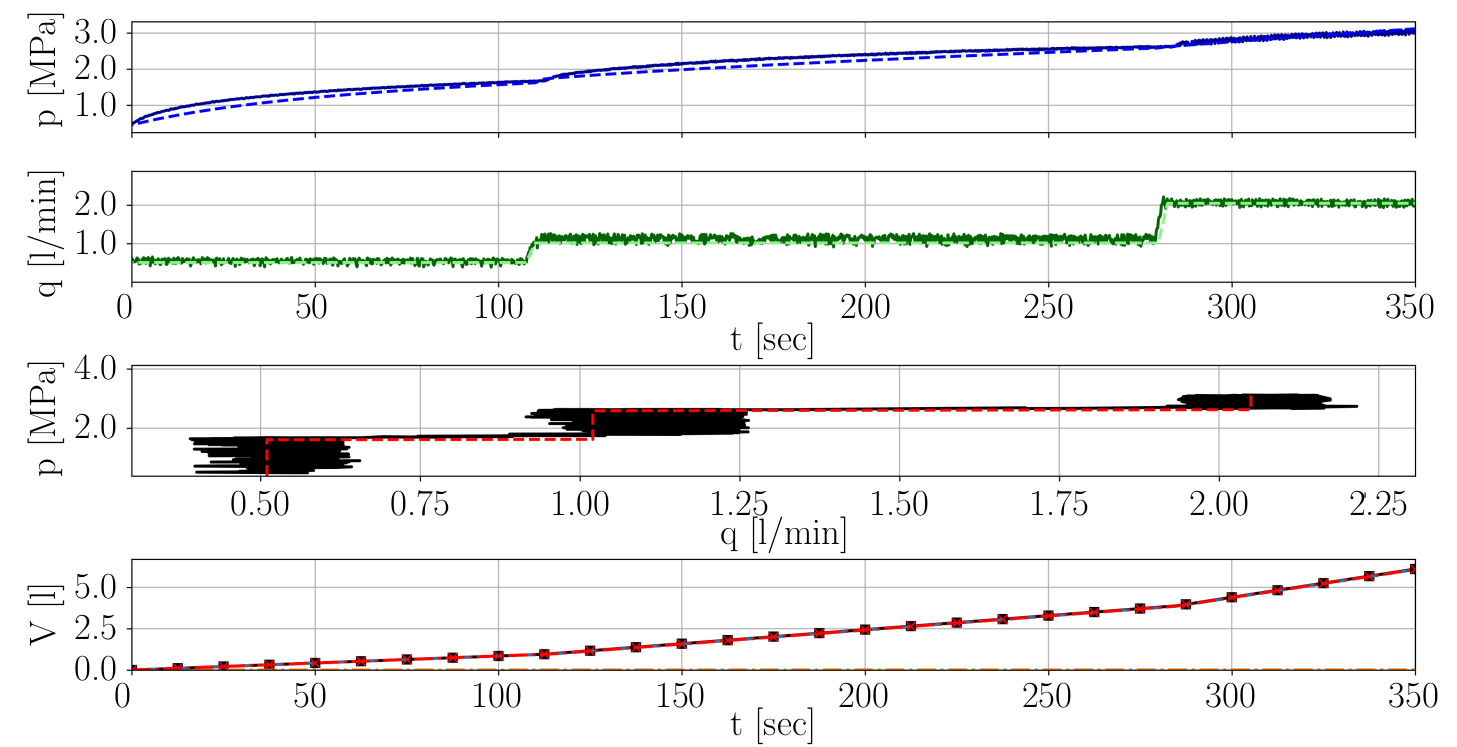
\includegraphics[width=1.0\textwidth]{./figures/data_management_reiche_zeche_40_6.png}
\end{center}
\caption{Visualisation of data obtained from the pre-compiled executable used for inverse analysis computations of pumping tests performed at Reiche Zeche at a depth of $40.6\,$m.}
\label{fig:DataReicheZeche}
\end{figure}

The uploaded data set contains two compiled executables for simulations to fit experimental data for the Reiche Zeche fracture characterization tests and to reproduce the non-linear response throughout harmonic testing of a single fracture on the laboratory scale like described in section \ref{sec:mex09}. The folder includes executables, input files and the used discretization in terms of meshing files, required to perform the simulations. README.txt files provide further informations how to start the simulations.

\begin{table}[!ht]
\caption{MEX 3-3: Reiche Zeche Data}
\label{tab:dms-mex3-3}
\small
\begin{tabular}{R{3cm}|L{7cm}}
\hline
%
Data label & GeomInt | UoS | Data Set Reiche Zeche \\
URI &  https://galilei.isr.uni-stuttgart.de/gitlab/schmidt/geomint\\
Subject  &  Non-linear hydro-mechanics / fracture flow\\
Type of data  &  executable, mesh input, parameter input\\
Dataquality  &  quality assured data \\
Status of data  &  unprocessed data\\
Dataformat  & txt, msh, linux executable\\
Creators  &  University of Stuttgart, Institute of Applied Mechancis - Continuum Mechanics, Pfaffenwaldring 7, 70569 Stuttgart\\
Source/Origin & In-house code \\
Publisher  &  University of Stuttgart, Institute of Applied Mechancis - Continuum Mechanics, Pfaffenwaldring 7, 70569 Stuttgart \\
Rights holders & University of Stuttgart, Institute of Applied Mechancis - Continuum Mechanics, Pfaffenwaldring 7, 70569 Stuttgart \\
Contributors &  University of Stuttgart, Institute of Applied Mechancis - Continuum Mechanics, Patrick Schmidt and Holger Steeb\\
Time or Period of creation &  2018-2019\\
Language of the content &  English\\
Update policy &  stored data is final\\
Access permissions &  full access\\
%
\hline
\end{tabular}
\end{table}
\clearpage
%------------------------------------------------------------------------

\begin{comment}
%-------------------
\begin{table}[!ht]
\footnotesize
\centering
\caption{MEX 0-1a: Data Management}
\label{tab:dms-mex0-1}
\begin{tabular}{|L{0.5cm}|L{1cm}|L{2cm}|L{3cm}|L{1cm}|} 
\hline
%..................
\rowcolor{cyan!50}
 & Methods & Codes/Reference & Files & Analysis \\ \hline
 & EXP & \cite{} & Files & Analysis \\ \hline
 & LEM & Codes & Files & Analysis \\ \hline
 & DEM & UDEC & Files & Analysis \\ \hline
 & FEM & OGS-6 & Benchmark collection\footnote{\url{https://www.opengeosys.org/docs/benchmarks/phase-field/phasefield/}} & Analysis \\ \hline
%..................
\end{tabular}
\end{table}
\normalsize
%-------------------
\end{comment}